\documentclass[11pt]{article}
\usepackage[a4paper,margin=2.05cm]{geometry}
\usepackage{amsmath,amssymb,booktabs,graphicx,float,xcolor,hyperref,longtable,array,enumitem,fancyhdr}
\usepackage{algorithm}
\usepackage{algpseudocode}
\usepackage{microtype}
\usepackage{xurl}
% Figures are the deck's figures, copied verbatim from presentation/figures/.
\graphicspath{{figures_v2/}{figures/}}
\hypersetup{colorlinks=true,linkcolor=blue,urlcolor=blue,citecolor=blue}
\definecolor{xjtblue}{HTML}{173F6B}
\setlength{\headheight}{22pt}
\pagestyle{fancy}
\fancyhf{}
\fancyhead[L]{\small\color{xjtblue}MTH321 Project 2}
\fancyhead[R]{\small\color{xjtblue}MTH321}
\fancyfoot[C]{\thepage}
\renewcommand{\headrulewidth}{0.55pt}
\renewcommand{\headrule}{\hbox to\headwidth{\color{xjtblue}\leaders\hrule height \headrulewidth\hfill}}
\fancypagestyle{cover}{
  \fancyhf{}
  \fancyhead[L]{\small\color{xjtblue}MTH321 Project 2}
  \fancyhead[R]{\small\color{xjtblue}MTH321}
  \renewcommand{\headrulewidth}{0.55pt}
}
\newcommand{\todo}[1]{\textcolor{red!70!black}{\textbf{[#1]}}}
\newcommand{\epsr}{\varepsilon_r}
\newcommand{\epseff}{\varepsilon_{\mathrm{eff}}}
\newcommand{\Cair}{C_{\mathrm{air}}}   % symbol
\newcommand{\Zzero}{Z_0}
\newcolumntype{L}[1]{>{\raggedright\arraybackslash}p{#1}}
% Numbers shared with the slides: presentation/numbers.tex plus the extra
% macros written by report/build_numbers.py.  Nothing below is hand-typed.
% Generated by presentation/make_figures.py -- do not edit by hand.
% Every number on the slides comes from tables/*.csv or code_hardened/results/*.json.

\newcommand{\CRef}{120.467}
\newcommand{\CRefPOne}{120.4673}
\newcommand{\CRefPTwo}{120.4670}
\newcommand{\RefAgree}{2.9\times10^{-6}}
\newcommand{\CFinal}{120.620}
\newcommand{\CFinalAbs}{0.153}
\newcommand{\ErrSeven}{0.127}
\newcommand{\ErrSix}{0.282}
\newcommand{\DeltaSeven}{0.156}
\newcommand{\DofSeven}{362{,}112}
\newcommand{\DofFive}{22{,}944}
\newcommand{\CAir}{35.968}
\newcommand{\CAirRef}{35.946}
\newcommand{\OrderPOne}{1.16}
\newcommand{\OrderPTwo}{1.15}
\newcommand{\GradedDof}{139{,}426}
\newcommand{\GradedErr}{0.017}
\newcommand{\GradedRatio}{7.6}
\newcommand{\GradedDofFrac}{39}
\newcommand{\TolDisc}{6.3\times10^{-3}}
\newcommand{\EpsEff}{3.3535}
\newcommand{\EpsRef}{3.3513}
\newcommand{\EpsErr}{0.07}
\newcommand{\ZFinal}{50.642}
\newcommand{\ZRef}{50.690}
\newcommand{\ZErrAbs}{0.048}
\newcommand{\ZErrPct}{0.09}
\newcommand{\ZHJ}{50.201}
\newcommand{\ZIPC}{49.393}
\newcommand{\ZBenchGap}{0.81}
\newcommand{\CheckCount}{23}
\newcommand{\TruncThree}{2.49}
\newcommand{\TruncFive}{0.71}
\newcommand{\TruncEight}{0.18}
\newcommand{\TruncFine}{0.036}
\newcommand{\RatioChange}{1.23}

% ---- extras written by report/build_numbers.py (same sources) ----
\newcommand{\ErrThree}{3.16}
\newcommand{\ErrFour}{1.40}
\newcommand{\ErrFive}{0.63}
\newcommand{\DeltaThree}{--}
\newcommand{\DeltaFour}{1.731}
\newcommand{\DeltaFive}{0.770}
\newcommand{\DeltaSix}{0.346}
\newcommand{\DofThree}{1{,}512}
\newcommand{\DofFour}{5{,}840}
\newcommand{\DofSix}{90{,}944}
\newcommand{\ElemsSeven}{720{,}896}
\newcommand{\CAirErr}{0.06}
\newcommand{\CornerAlpha}{0.52}
\newcommand{\CornerAlphaLo}{0.47}
\newcommand{\CornerAlphaHi}{0.61}
\newcommand{\CornerTwoAlpha}{1.03}
\newcommand{\GradedBTwo}{1.087}
\newcommand{\GradedBThree}{0.270}
\newcommand{\GradedBFour}{0.069}
\newcommand{\GradedBFive}{0.017}
\newcommand{\PlateauOne}{4.02}
\newcommand{\PlateauTwo}{3.91}
\newcommand{\PlateauThree}{4.12}
\newcommand{\TolAlgebraicAtCoarse}{2.1\times10^{-2}}
\newcommand{\TolAlgebraicFloor}{1\times10^{-16}}

\newcommand{\MMSLTwoFit}{1.9956}
\newcommand{\MMSEnergyFit}{0.9983}
\newcommand{\RefSlopeROne}{0.6383}
\newcommand{\RefSlopeRTwo}{0.6230}
\newcommand{\HJDiscrepancyFEM}{0.88}
\newcommand{\HJDiscrepancyIPC}{1.61}

\newcommand{\coverlogo}{%
  \IfFileExists{figures/xjtlu_logo_blue.pdf}%
    {
\includegraphics[width=0.72\textwidth]{figures/xjtlu_logo_blue.pdf}}%
    {\begin{minipage}{0.8\textwidth}\centering\vspace{1.2cm}
       {\color{xjtblue}\LARGE\bfseries Xi'an Jiaotong-Liverpool University}\par
       \vspace{0.9cm}\end{minipage}}}

\begin{document}
\hypersetup{pageanchor=false}
\begin{titlepage}
\thispagestyle{cover}
\centering
\vspace*{0.45cm}
\coverlogo

\vspace{1.35cm}
{\color{xjtblue}\rule{0.86\textwidth}{1.1pt}}

\vspace{0.85cm}
{\Huge\bfseries 2D Finite Element Analysis\\[0.18cm] of a Microstrip Transmission Line\par}
\vspace{0.45cm}

\vspace{0.85cm}
{\color{xjtblue}\rule{0.86\textwidth}{0.55pt}}

\vspace{0.9cm}
{\large\bfseries MTH321 Project 2\par}

\vspace{1.0cm}
{\large\bfseries Group and student details\par}
\vspace{0.35cm}
\renewcommand{\arraystretch}{1.35}
\begin{tabular}{@{}ll@{}}
Group name & Group C\\
Student names and IDs & Chuqiao Tang (2360692)\\
 & Jinyu Ma (2363433)\\
 & Muqing Xu (2362900)\\
 & Shuoran Fu (2362626)\\
 & Taiqi Zhang (2363684)\\
 & Yujia Ding (2362094)
\end{tabular}

\vfill
{\normalsize October 2026\par}
\vspace{0.2cm}
\end{titlepage}
\hypersetup{pageanchor=true}

\pagenumbering{roman}
\begin{abstract}
A finite-element capacitance is only useful if the distance to its limit is known.
We compute the capacitance of a $3.0\,\mathrm{mm}$-wide, $0.035\,\mathrm{mm}$-thick trace on
a $1.6\,\mathrm{mm}$ FR-4 substrate with conforming triangular $P_1$ elements, and we spend
most of the report establishing that limit rather than the number.

The solver is pinned down before anything is measured. $\CheckCount$ analytic
configurations are reproduced to roundoff, a manufactured solution returns the expected
orders, and a layered interface keeps its normal flux continuous to $2.3\times10^{-13}$,
so any remaining error is discretisation. Two independent routes, Richardson extrapolation
of the project's own $P_1$ sequence and a separately written scikit-fem $P_2$ solve, then
place the limit at $C_{\mathrm{ref}}=\CRef\,\mathrm{pF/m}$; they agree to
$\RefAgree$ relative.

Against that limit the usual convergence indicator is misleading. At M7 the change from
M6 is $\DeltaSeven\%$, while the actual distance from the limit is $\ErrSeven\%$; the two
differ by the factor $2^{p}-1=\RatioChange$, which a shrinking difference conceals
unless $p$ is known. The measured order is $p=\OrderPOne$ for $P_1$ and $\OrderPTwo$ for
$P_2$: doubling the polynomial degree does not buy an order, because the rate is set by the
conductor corner and not by the basis.

Corner grading restores the order. Seven rounds of geometric refinement on the M5
background reach $\GradedErr\%$ with $\GradedDof$ unknowns, which is
$\GradedRatio\times$ closer than M7 at $\GradedDofFrac\%$ of its degrees of freedom. The
truncation of the $8H$ box contributes $\TruncEight\%$, the same size as the
discretisation error, and the algebraic error sits thirteen orders of magnitude below
both, so the budget belongs entirely to the corner.

The submitted values are $C=\CFinal\,\mathrm{pF/m}$, which is $\CFinalAbs\,\mathrm{pF/m}$
or $\ErrSeven\%$ from the extrapolated limit, and $\Cair=\CAir\,\mathrm{pF/m}$ on exactly
the same M7 mesh, giving
$\epseff=\EpsEff$ (against an exact $\EpsRef$, an error of $\EpsErr\%$) and
$\Zzero=\ZFinal\,\Omega$ (against $\ZRef\,\Omega$, a difference of
$\ZErrAbs\,\Omega$). The ratio cancels most of the common bias, which is why the
engineering quantities are roughly twice as accurate as the capacitance they come from.
\end{abstract}
\tableofcontents
\newpage
\pagenumbering{arabic}

\section{Introduction}
\subsection{What is delivered, and what is not}
A microstrip cross-section is specified by geometry and permittivity, and the quantity an
engineer wants is the characteristic impedance. Under a lossless quasi-TEM model that
impedance follows from a matched pair of capacitances: the dielectric one, $C$, and the
same geometry with every field element assigned air, $\Cair$. The deliverable of this
project is therefore a number and, with equal weight, the distance from its limit. A
single finite-element value that happens to sit near $50\,\Omega$ is not a result; nor is
agreement with an empirical formula, nor a claim of convergence inferred from two meshes
that happen to agree.

The work is organised around four questions: whether the solver is right (Section~3), what
the limit is (Section~4), how far the submitted mesh sits from it and what controls that
distance (Sections~5--7), what an adaptive strategy would add (Section~8), and what else
contributes at the same size (Sections~9--10). The final quantities follow in Section~11.

\subsection{Geometry, materials and notation}
The nominal geometry is a copper trace of width $w=3.0\,\mathrm{mm}$ and thickness
$t=0.035\,\mathrm{mm}$ on a substrate of height $H=1.6\,\mathrm{mm}$ and relative
permittivity $\epsr=4.4$, as listed in Table~\ref{tab:parameters} and drawn in
Figure~\ref{fig:geometry}. All computations use SI units internally. The computational
rectangle has half-width $W$ and top-boundary height $H_{\mathrm{air}}$, measured from the
ground, so $x\in[-W,W]$ and $y\in[0,H_{\mathrm{air}}]$; the final engineering domain uses
$W/H=H_{\mathrm{air}}/H=8$ after the truncation study of Section~9.

\begin{table}[H]
\centering
\small
\caption{Physical and computational parameters for the final microstrip model.}
\label{tab:parameters}
\begin{tabular}{@{}lll@{}}
\toprule
Quantity & Value & Meaning\\
\midrule
$H$ & $1.6\times 10^{-3}\,\mathrm{m}$ & substrate height\\
$w$ & $3.0\times 10^{-3}\,\mathrm{m}$ & trace width\\
$t$ & $3.5\times 10^{-5}\,\mathrm{m}$ & trace thickness\\
$\epsr$ & $4.4$ & substrate relative permittivity\\
$V_0$ & $1\,\mathrm{V}$ & trace potential\\
$W/H$ & $8$ & final half-width ratio\\
$H_{\mathrm{air}}/H$ & $8$ & final height ratio\\
\bottomrule
\end{tabular}
\end{table}

\begin{figure}[htbp]
\centering
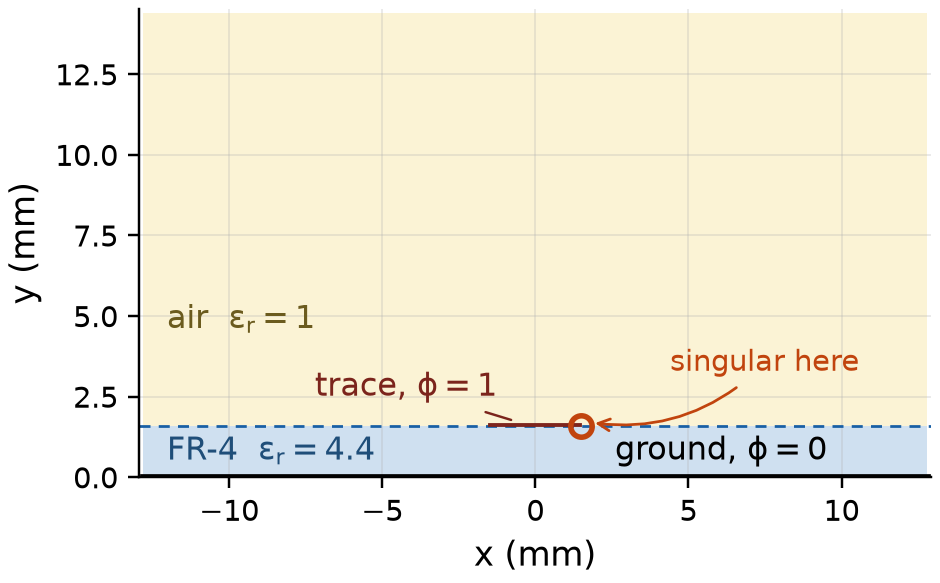
\includegraphics[width=0.78\textwidth]{fig01_geometry.png}
\caption{The cross-section. The substrate occupies $0<y<H$, air lies above it, and the
trace interior is removed from the field domain so that its surface is an internal
Dirichlet boundary. The circle marks the corner where the conductor edge meets the
dielectric interface; it is the only place in the problem where the solution is not
smooth, and Sections~6--7 are about it.}
\label{fig:geometry}
\end{figure}

\section{Physical and Mathematical Model}
\subsection{Governing equation and boundary conditions}
The field domain $\Omega$ is the computational rectangle with the conductor interior
removed. The only unknown is the electric potential $\phi(x,y)$ in volts, and the material
coefficient $\varepsilon(x,y)=\varepsilon_0\epsr(x,y)$ in F/m is piecewise constant:
$4.4\varepsilon_0$ in the substrate and $\varepsilon_0$ in air. With no free volume charge,
\begin{equation}
 -\nabla\cdot(\varepsilon \nabla \phi)=0 \qquad \text{in }\Omega ,
 \label{eq:pde}
\end{equation}
with essential data
\[
\phi=V_0 \quad \text{on the signal trace},\qquad
\phi=0 \quad \text{on the ground plane},
\]
and a homogeneous Neumann condition $\varepsilon\nabla\phi\cdot n=0$ on the artificial top
and side walls $\Gamma_{\rm far}$, where $n$ is the outward unit normal. The electric
field is $\mathbf E=-\nabla\phi$ and the displacement is $\mathbf D=\varepsilon\mathbf E$;
the zero-flux condition therefore prescribes zero normal displacement on the artificial
walls, which is an approximation whose cost is measured in Section~10. Across the
air--substrate interface the exact conditions are continuity of potential and balance of
normal displacement flux. The electrostatic energy per unit length is
\begin{equation}
W_e(\phi)=\frac12\int_\Omega\varepsilon(x,y)|\nabla\phi|^2\,d\Omega ,
\label{eq:energy}
\end{equation}
and the capacitance follows from it. Positive discontinuous coefficients of this kind are
naturally treated in a variational formulation with separate integration over each
material region, as discussed by Hackbusch~\cite[Sec.~10.1]{hackbusch2017}.

\subsection{Weak form and well-posedness}
Let $\partial\Omega$ denote the entire boundary and $\Gamma_D$ the union of the trace and
ground Dirichlet boundaries; $H^1(\Omega)$ contains square-integrable functions with
square-integrable first weak derivatives. The affine trial space and homogeneous test
space are
\[
V_g=\{u\in H^1(\Omega):u=V_0 \text{ on the trace},\ u=0 \text{ on the ground}\},
\qquad
\mathcal V=\{v\in H^1(\Omega):v=0 \text{ on }\Gamma_D\}.
\]
Multiplying~\eqref{eq:pde} by $v\in\mathcal V$ and integrating by parts, with $ds$
denoting boundary arclength, the boundary term vanishes because $v=0$ on $\Gamma_D$ and
the prescribed normal flux is zero elsewhere. The weak problem is: find $\phi\in V_g$ such
that
\begin{equation}
a(\phi,v):=\int_{\Omega}\varepsilon \nabla\phi\cdot\nabla v\,d\Omega=0
\qquad\forall v\in\mathcal V .
\label{eq:weak}
\end{equation}
The bilinear form is continuous and coercive even across the dielectric jump, since
$\varepsilon_0\le\varepsilon\le4.4\varepsilon_0$ everywhere:
\[
|a(u,v)|\le4.4\varepsilon_0\|\nabla u\|_{L^2}\|\nabla v\|_{L^2},
\qquad a(v,v)\ge\varepsilon_0\|\nabla v\|_{L^2}^2 .
\]
Because $\Gamma_D$ has positive boundary measure, the Poincar\'e inequality holds on
$\mathcal V$, so the gradient seminorm is a norm there. Taking an $H^1$ lifting $g$ of the
prescribed data and writing $\phi=g+u$ with $u\in\mathcal V$ gives a bounded load
$\ell(v)=-a(g,v)$, and Lax--Milgram supplies existence and uniqueness. The Dirichlet
constraints also remove the constant nullspace of the pure-Neumann problem: two solutions
differ by a constant, and a zero Dirichlet trace forces that constant to vanish. The
argument is the standard one for elliptic problems, as in
Hackbusch~\cite[Sec.~7.2]{hackbusch2017} and Quarteroni~\cite[Secs.~3.4 and 4.2]{quarteroni2017}.

\subsection{Discretisation, assembly and capacitance extraction}
The discrete space $\mathcal V_h\subset\mathcal V$ uses conforming triangles and
continuous functions that are affine on each triangle, following
Quarteroni~\cite[Sec.~4.5]{quarteroni2017} and Hiptmair~\cite[Sec.~2.4]{hiptmair2025}.
Writing $\phi_h=\sum_j\Phi_jN_j$ with nodal basis functions $N_j$, the stiffness entries
are
\begin{equation}
K_{ij}=\int_{\Omega}\varepsilon \nabla N_i\cdot \nabla N_j\,d\Omega .
\label{eq:stiffness}
\end{equation}
On a material-conforming triangle of area $|K|$ and coefficient $\varepsilon_K$ the basis
gradients are constant, so the element contribution
$K^K_{ij}=\varepsilon_K|K|\nabla N_i\cdot\nabla N_j$ is integrated exactly; the assembly is
therefore exact to roundoff, and the only errors left are discretisation errors. This is
the property that makes the verification of Section~3 meaningful: a residual or a matrix
identity cannot be ``approximately'' satisfied.

Prescribed values are imposed by elimination. With $\Phi_D$ the prescribed nodal values and
$\Phi_F$ the unknowns, the reduced system is
\begin{equation}
K_{FF}\Phi_F=b_F,\qquad b_F=-K_{FD}\Phi_D ,
\label{eq:elimination}
\end{equation}
which is symmetric positive definite. The full reaction vector $r=K\Phi$ carries the
surface charge per unit length on the Dirichlet nodes, so the two capacitances are
\begin{equation}
C_E=\frac{2W_e}{V_0^2},\qquad C_Q=\frac{|Q_{\mathrm{trace}}|}{|V_0|},
\label{eq:capacitance}
\end{equation}
where $Q_{\rm trace}$ is the sum of the trace reactions. Agreement of $C_E$ and $C_Q$ tests
that energy integration and reaction extraction use the same operator; it is a consistency
check, not an accuracy check, a distinction that matters in Appendix~A.

\begin{algorithm}[H]
\caption{Microstrip $P_1$ FEM solver}\label{alg:fem}
\begin{algorithmic}[1]
\Require Material-conforming mesh $\mathcal T_h$, geometry, $\varepsilon_K$ and voltage $V_0$
\State Generate the study mesh, or load the exact frozen mesh for a matched replay.
\State Verify the trace hole, interface, element regions and trace/ground/far boundary sets.
\State Set $D=D_{\rm trace}\cup D_{\rm ground}$, $F=\{\text{all nodes}\}\setminus D$.
\State Initialise $\Phi_D=V_0$ on the trace and $\Phi_D=0$ on ground; set $K=0$.
\For{each triangle $K_e\in\mathcal T_h$}
\State Compute $|K_e|$ and its three constant basis gradients.
\State Assemble $\varepsilon_{K_e}|K_e|\nabla N_i\cdot\nabla N_j$ into the sparse matrix.
\EndFor
\State Solve $K_{FF}\Phi_F=-K_{FD}\Phi_D$ by a sparse direct solver.
\State Evaluate $\nabla\phi_h$, $W_e$, $C_E=2W_e/V_0^2$ and reactions $r=K\Phi$.
\State Sum trace reactions to obtain $Q_{\rm trace}$ and $C_Q=|Q_{\rm trace}|/|V_0|$.
\State Check bounds, symmetry, residual, charge balance and $C_E/C_Q$ consistency.
\Ensure Potential, capacitances and diagnostics; failed checks disqualify interpretation.
\end{algorithmic}
\end{algorithm}

The recorded environment uses Python 3.13 with scikit-fem 12.0.2 for mesh topology,
quadrature and the manufactured-solution basis, and SciPy sparse direct solves. Our own
code defines the trace hole, the material and boundary tags, the grading and the
capacitance extraction; those parts are tested separately from the library, in
\path{code_hardened/}, so that a library change cannot silently move the answer.

\section{Solver Verification}
\subsection{Twenty-three analytic configurations}
Before any mesh study, the operator and the extraction are checked against cases whose
answer is known in closed form. Figure~\ref{fig:checks} groups the configurations into
five families: a uniform field against $\phi=y/d$ for $\epsr=1$ and $4.4$; a parallel-plate
capacitance against $\varepsilon_0\epsr A/d$; the two-dimensional series-layer
capacitance; continuity of the normal displacement across an interface; and the total
induced charge implied by charge balance. Each configuration is run through the production
assembly and the production extraction, not through a test-only copy.

\begin{figure}[htbp]
\centering
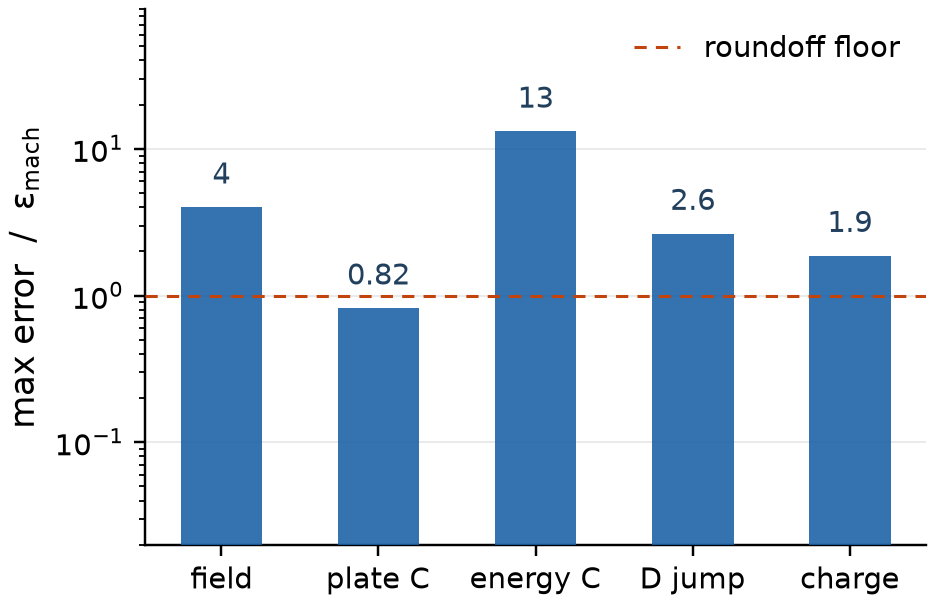
\includegraphics[width=0.78\textwidth]{fig02_checks.png}
\caption{Worst error in each family of analytic checks, in units of machine epsilon
($\CheckCount$ configurations in total). The dashed line is the roundoff floor. Every
family sits within a factor of about thirteen of it, so the discrete operator reproduces
the exact identities of the model rather than approximating them.}
\label{fig:checks}
\end{figure}

All $\CheckCount$ checks pass, the worst relative error being about
$13\varepsilon_{\rm mach}$. Two consequences are used later. No part of the reported error
can be attributed to assembly, extraction or the Dirichlet treatment in the
constant-coefficient case, so what remains is discretisation and truncation. And a check
that fails at this level is a coding error rather than a modelling choice, which is why the
guard stays in the pipeline instead of being run once.

\subsection{Manufactured solution}
A manufactured solution measures the discretisation error directly and compares the
observed rate with the smooth-solution estimate. On the unit square with zero Dirichlet
data we impose $u(x,y)=\sin(\pi x)\sin(\pi y)$ and
$f=2\pi^2\sin(\pi x)\sin(\pi y)$ in $-\Delta u=f$, and refine five times. Table~\ref{tab:mms}
reports the $L^2$ and energy errors together with the pairwise orders
$p_i=\log(E_{i-1}/E_i)/\log(h_{i-1}/h_i)$.

\begin{table}[H]
\centering
\small
\caption{Consecutive manufactured-solution refinements. $N_T$ is the triangle count and
$r_F$ the free-system algebraic residual; all levels use a sparse direct solve.}
\label{tab:mms}
\begingroup
\setlength{\tabcolsep}{3pt}
\begin{tabular}{@{}lrrrrrrrr@{}}
\toprule
Level & $N_T$ & DOFs & $h_{\max}$ & $\|e\|_{L^2}$ & $\|e\|_E$ & $\|r_F\|_\infty$ & $p_{L^2}$ & $p_E$\\
\midrule
2 ($h$) & 32 & 25 & 0.35355 & $7.596\times10^{-2}$ & $8.397\times10^{-1}$ & $3.331\times10^{-16}$ & -- & --\\
3 ($h/2$) & 128 & 81 & 0.17678 & $2.041\times10^{-2}$ & $4.320\times10^{-1}$ & $5.551\times10^{-16}$ & 1.896 & 0.959\\
4 ($h/4$) & 512 & 289 & 0.08839 & $5.201\times10^{-3}$ & $2.176\times10^{-1}$ & $9.021\times10^{-16}$ & 1.972 & 0.989\\
5 ($h/8$) & 2048 & 1089 & 0.04419 & $1.307\times10^{-3}$ & $1.090\times10^{-1}$ & $1.457\times10^{-15}$ & 1.993 & 0.997\\
6 ($h/16$) & 8192 & 4225 & 0.02210 & $3.270\times10^{-4}$ & $5.451\times10^{-2}$ & $2.368\times10^{-15}$ & 1.998 & 0.999\\
\bottomrule
\end{tabular}

\endgroup
\end{table}

Least-squares fits over the finest three levels give $p_{L^2}=\MMSLTwoFit$ and
$p_E=\MMSEnergyFit$, and the largest residual listed is $2.4\times10^{-15}$, far below the
acceptance level $\|r_F\|_\infty<10^{-10}$ used throughout the project. The protocol is the
one of Hiptmair~\cite[Sec.~3.8]{hiptmair2025}, and the rates are the ones Quarteroni predicts
for these elements~\cite[Sec.~4.5]{quarteroni2017}. What the table supports is the
implementation that was tested, not the microstrip geometry; the geometry tags carry their
own test, and the corner behaviour of Section~6 is measured rather than assumed.

\subsection{Layered interface}
The layered problem checks the treatment of a discontinuous coefficient, which is the one
feature the manufactured solution does not exercise. On the unit square, with $a=1$ for
$x<1/2$ and $a=10$ for $x>1/2$ and $f=0$, the exact solution is
\[
u_*(x)=\begin{cases}20x/11,&x\le1/2,\\(2x+9)/11,&x\ge1/2,\end{cases}
\]
for which both traces equal $10/11$ at the interface while the gradients are $20/11$ and
$2/11$, so the physical flux $q_*=-a\partial_xu_*=-20/11$ is continuous. The test calls the
production \texttt{assemble\_stiffness} with relative coefficients 1 and 10 and divides out
the common $\varepsilon_0$.

\begin{table}[H]\centering\small
\caption{Layered verification using the production assembly. Odd $N$ leaves the interface
unresolved and tags elements by centroid: it is a negative control, not an acceptable
method.}
\begin{tabular}{@{}lcrrr@{}}
\toprule
$N$ & Fitted? & DOFs & $\|u_h-u_*\|_\infty$ (nodes) & $\|q_h-q_*\|_{L^2}$\\
\midrule
4 & yes & 25 & 3.33e-16 & 3.18e-15\\
8 & yes & 81 & 8.88e-16 & 1.04e-14\\
16 & yes & 289 & 2.11e-15 & 3.86e-14\\
32 & yes & 1089 & 3.22e-15 & 9.15e-14\\
7 & no & 64 & 8.15e-02 & 1.07e+00\\
15 & no & 256 & 3.95e-02 & 5.80e-01\\
31 & no & 1024 & 1.94e-02 & 3.42e-01\\
\bottomrule
\end{tabular}
\label{tab:layered}
\end{table}

On fitted meshes the largest normal-flux jump is $2.28\times10^{-13}$, and the reduced
matrices are symmetric with a positive smallest eigenvalue. The negative control carries the
lesson. It holds a small residual and a symmetric positive matrix while its solution error is
ten orders of magnitude larger, so solving the discrete equations accurately says nothing
about whether the interface was represented. That is the failure mode a coefficient-jump bug
produces.

\begin{figure}[htbp]
\centering
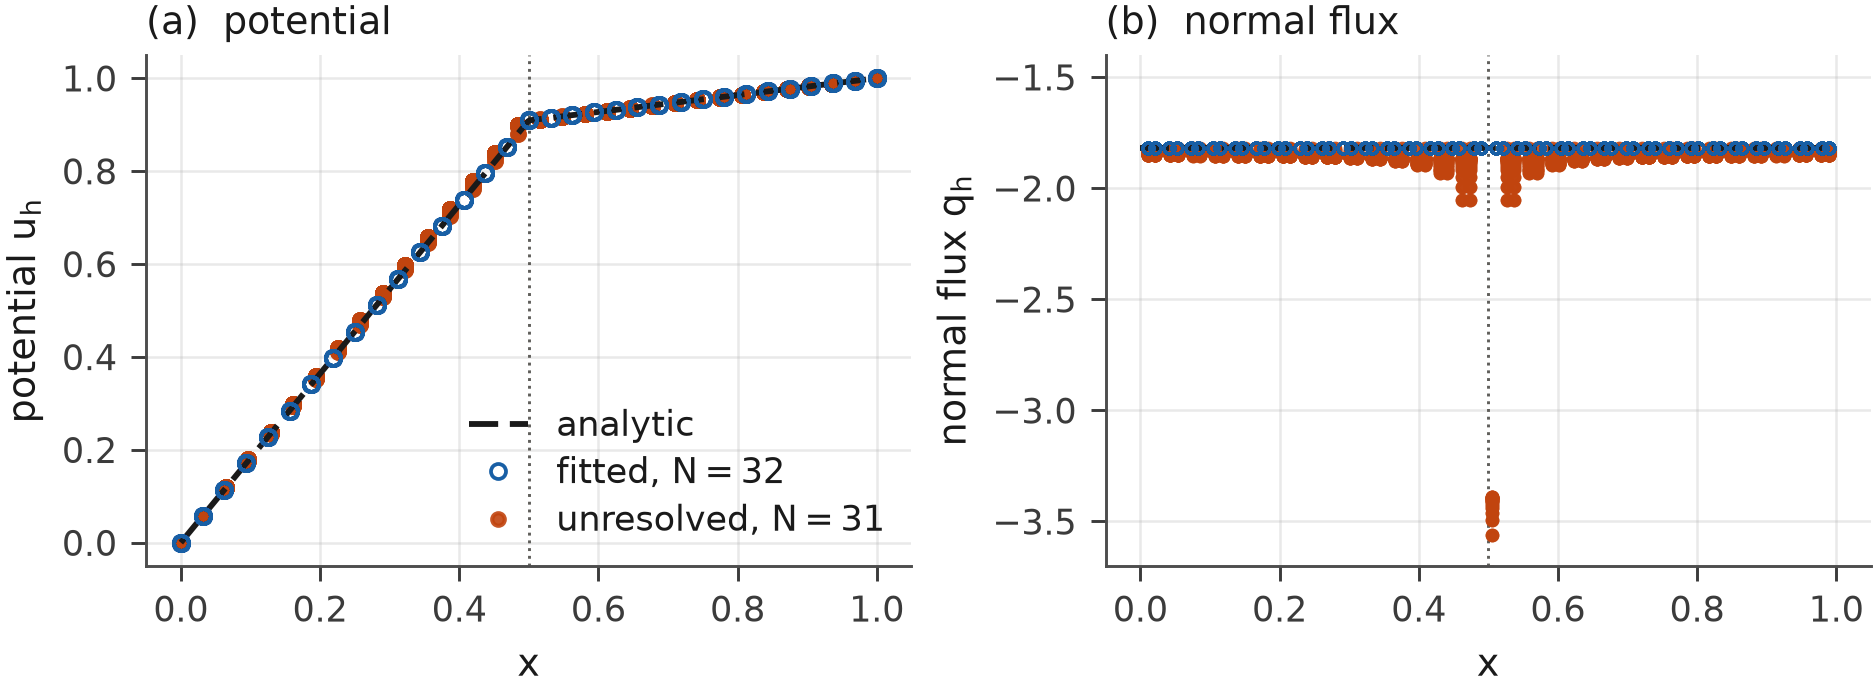
\includegraphics[width=\textwidth]{fig14_layered.png}
\caption{Layered interface with $a=1$ for $x<1/2$ and $a=10$ for $x>1/2$. The fitted mesh
($N=32$) reproduces the analytic potential and keeps the normal flux $q_h=-a\,\partial_x u_h$
at its exact value $-20/11$ on both sides of the interface. The unresolved control ($N=31$)
tracks the potential almost as well and yet its flux jumps to $-3.4$ at the interface, which
is the paired failure the table above records in numbers.}
\label{fig:layered}
\end{figure}

\subsection{The Dirichlet row on non-zero data}
The checks above all use boundary data with the ground at $0\,\mathrm{V}$, and so does the
production API, which hard-wires that value. On such data the ground columns of the
elimination shift $-K_{FD}\Phi_D$ are identically zero, so no test in the suite can see an
error confined to them. We therefore verified the row separately
(\path{code_hardened/boundary_row_audit.py}, commit \texttt{ccd2f37}) by building the same
system three independent ways: the shipped elimination, a textbook row replacement, and
the shipped solver shifted by a constant, on a layered box driven with $1\,\mathrm{V}$ on
the ground and $3\,\mathrm{V}$ on the trace.

The three constructions agree to $8.1\times10^{-16}$ of the applied voltage on the box and to
$7.8\times10^{-15}$ on the project mesh, the row-replacement solution matches the closed-form
series field to $1.1\times10^{-15}$, and one element is eliminated by hand in exact rational
arithmetic with error zero. Deleting the ground columns of the shift, which is the error the
observation is about, moves the same norm by $0.33\,\mathrm{V}$ on the box. On the project's
own mesh it moves the norm by $7.8\times10^{-15}\,\mathrm{V}$, which states the blind spot
quantitatively: it is real, and the ordinary suite cannot reach it.

\section{The Limit}
\subsection{Two independent routes}
Every error quoted in this report is an error against a limit, so the limit has to be fixed
before anything is measured. We use two routes that share neither element type nor code. The
first is the project's own $P_1$ sequence on the nested $8H$ meshes M3--M7, extrapolated with
the Richardson formula for a halving sequence,
\begin{equation}
C_{\rm ext}=C_k+\frac{C_k-C_{k-1}}{2^{p_C}-1},\qquad
p_C=\log_2\frac{C_{k-2}-C_{k-1}}{C_{k-1}-C_k},
\label{eq:richardson}
\end{equation}
which uses only the fact that successive differences shrink geometrically. The second is a
separately written $P_2$ solver built on scikit-fem's element and assembly, run on the same
mesh family, so that a shared bug in our own assembly would move only one of the two limits.

\begin{figure}[htbp]
\centering
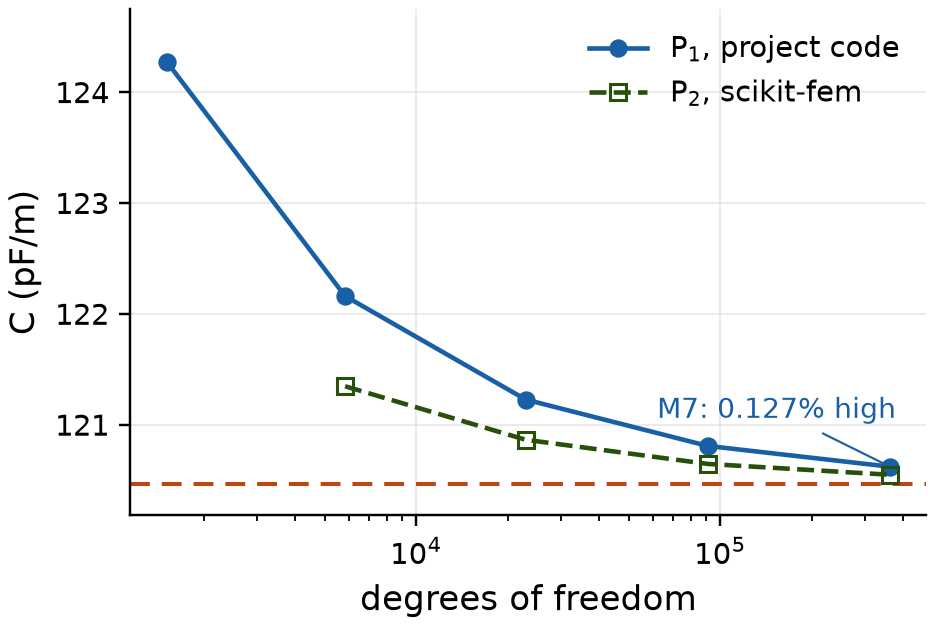
\includegraphics[width=0.78\textwidth]{fig03_reference.png}
\caption{Both families against the adopted limit. The two curves have different element
types, different unknowns and different codes, and both approach the same dashed line from
above, the $P_2$ sequence sitting closer to it at equal unknowns.}
\label{fig:reference}
\end{figure}

The two extrapolations are $\CRefPOne\,\mathrm{pF/m}$ ($P_1$) and $\CRefPTwo\,\mathrm{pF/m}$
($P_2$). They agree to $\RefAgree$ relative, which is three orders of magnitude below the
effect we are about to measure, so the adopted reference
\begin{equation}
C_{\rm ref}=\CRef\ \mathrm{pF/m}
\label{eq:cref}
\end{equation}
is not a fit to either family but the midpoint of two independent limits. This is the only
place where the two solvers are combined; every later number is produced by the $P_1$ code
alone.

\subsection{Why a single family would not be enough}
A single extrapolation cannot distinguish a limit from a slowly drifting artefact: if the
observed order is not constant, formula~\eqref{eq:richardson} reports a number whose
plausibility rests entirely on the assumption it uses. The second family supplies an
independent test of that assumption rather than more digits. What counts is that the two
answers agree although their orders differ slightly, $\OrderPOne$ against $\OrderPTwo$
(Section~6): both families are limited by the same non-smooth feature, so both extrapolations
head for the same limit, yet neither has reached the asymptotic regime in which the nominal
order would apply.

\section{What the Old Metric Measured}
\subsection{Change is not error}
The convergence indicator used earlier in the project was the relative change between
consecutive meshes, $dC_k=|C_k-C_{k-1}|/|C_k|$. At M7 it is $\DeltaSeven\%$, below the
$\pm0.1\%$ band the specification suggests, and that was read as convergence. Measured
against the reference of Section~4, the distance is $\ErrSeven\%$, more than twice as large.

\begin{figure}[htbp]
\centering
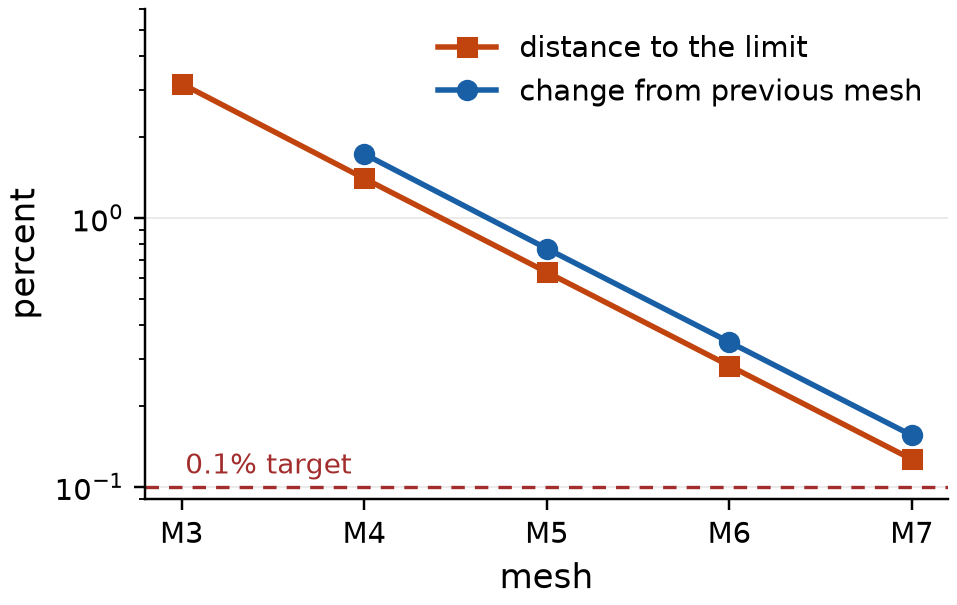
\includegraphics[width=0.78\textwidth]{fig04_metric.png}
\caption{The two quantities the report has to keep apart. The change from the previous mesh
falls below the $0.1\%$ target at M6--M7 while the distance to the limit is still about
$0.13\%$. A declining difference says the sequence is settling; it does not say how far
from its limit it is.}
\label{fig:metric}
\end{figure}

The relation between the two is fixed by the order. For a sequence with error
$e_k\propto h_k^{p}$ and mesh halving,
\[
dC_k\simeq(2^{p}-1)\,e_k ,
\]
so the change is the error multiplied by $2^{p}-1$. With $p=\OrderPOne$ that factor is
$\RatioChange$, which reproduces $\DeltaSeven/\ErrSeven$ to the quoted digits. The factor is
below one here, so the change \emph{understates} the error; for $p>1$ it would overstate it.
Without an estimate of $p$, a shrinking difference therefore bounds nothing.

\begin{table}[H]
\centering
\small
\caption{The uniform sequence against the reference of~\eqref{eq:cref}. The last two
columns are the two quantities of Figure~\ref{fig:metric}: the change from the previous
mesh, and the actual distance from the limit.}
\label{tab:uniform}
\begin{tabular}{@{}lrrrrr@{}}
\toprule
Mesh & DOFs & $C_E$ (pF/m) & change (\%) & error (\%) & $dC/\text{error}$\\
\midrule
M3 & \DofThree & 124.273 & \DeltaThree & \ErrThree & --\\
M4 & \DofFour & 122.159 & \DeltaFour & \ErrFour & 1.24\\
M5 & \DofFive & 121.225 & \DeltaFive & \ErrFive & 1.22\\
M6 & \DofSix & 120.807 & \DeltaSix & \ErrSix & 1.23\\
M7 & \DofSeven & \CFinal & \DeltaSeven & \ErrSeven & \RatioChange\\
\bottomrule
\end{tabular}
\end{table}

The ratio in the last column is constant at $\RatioChange$, as it must be while the sequence
stays in its geometric regime. That constancy is what makes the $0.127\%$ a measured distance
rather than an artefact of one particular mesh pair, since the same factor relates every
consecutive pair in the table.

\subsection{Consequence for the submitted value}
M7 misses the $\pm0.1\%$ band by a factor of about $1.27$, and the honest statement is that
the submitted capacitance is $\ErrSeven\%$ from its limit rather than converged to $0.1\%$.
Two responses are open: refine further, or change the discretisation so that the same number
of unknowns buys a smaller error. M8 would be roughly $1.4$ million unknowns behind a sparse
direct factorisation, so Section~7 takes the second route.

\section{Why the Order Is \texorpdfstring{$\OrderPOne$}{1.16}}
\subsection{Quadratic elements do not buy an order}
If the slow convergence were a property of the basis, doubling the polynomial degree would
remove it. Figure~\ref{fig:order} fits the error in $C$ against an $h$ proxy for both
families: the slope is $\OrderPOne$ for $P_1$ over $1.5$k--$362$k unknowns and
$\OrderPTwo$ for $P_2$ over $5.8$k--$362$k. The two are the same to the quoted digits.

\begin{figure}[htbp]
\centering
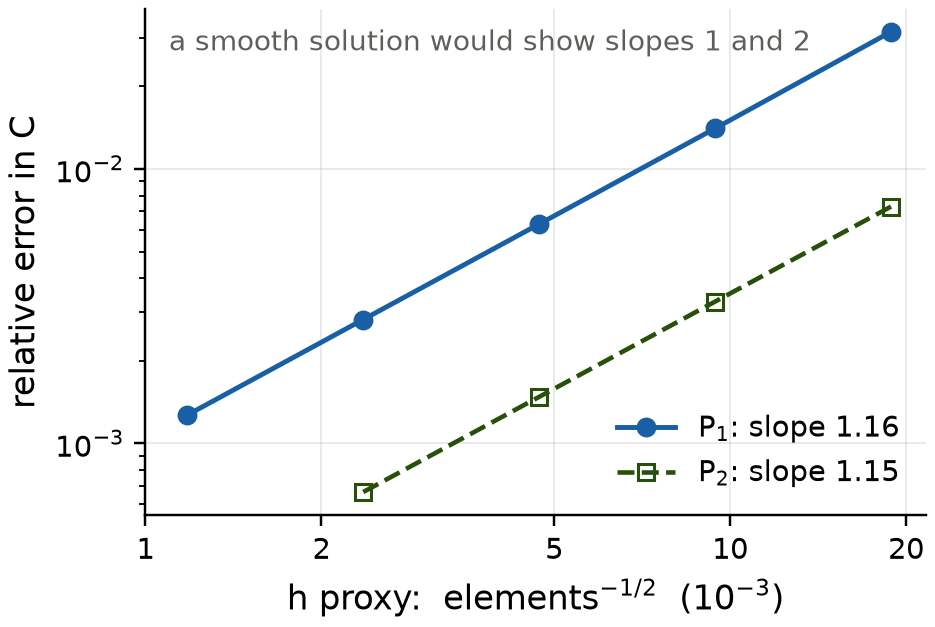
\includegraphics[width=0.68\textwidth]{fig05_order.png}
\caption{Error in $C$ against an $h$ proxy for both families. A smooth solution would give
slopes of one and two for $P_1$ and $P_2$ respectively; both families instead lie on nearly
the same line. The offset between them is a constant, not a rate.}
\label{fig:order}
\end{figure}

The diagnosis is unambiguous. A $P_2$ approximation has twice the local polynomial degree
and four times the unknowns per element, yet it converges at the same rate, so what limits
the error is the regularity of the solution and not the approximation space. Spending
unknowns on a richer basis is therefore not a cure; the error is generated at a point.
Figure~\ref{fig:field} shows the point. On the production domain the potential is flat over
most of the box and the field is confined to the dielectric within a few hundred micrometres
of the trace edge, so the unknowns that sit elsewhere have nothing to resolve.

\begin{figure}[t]
\centering
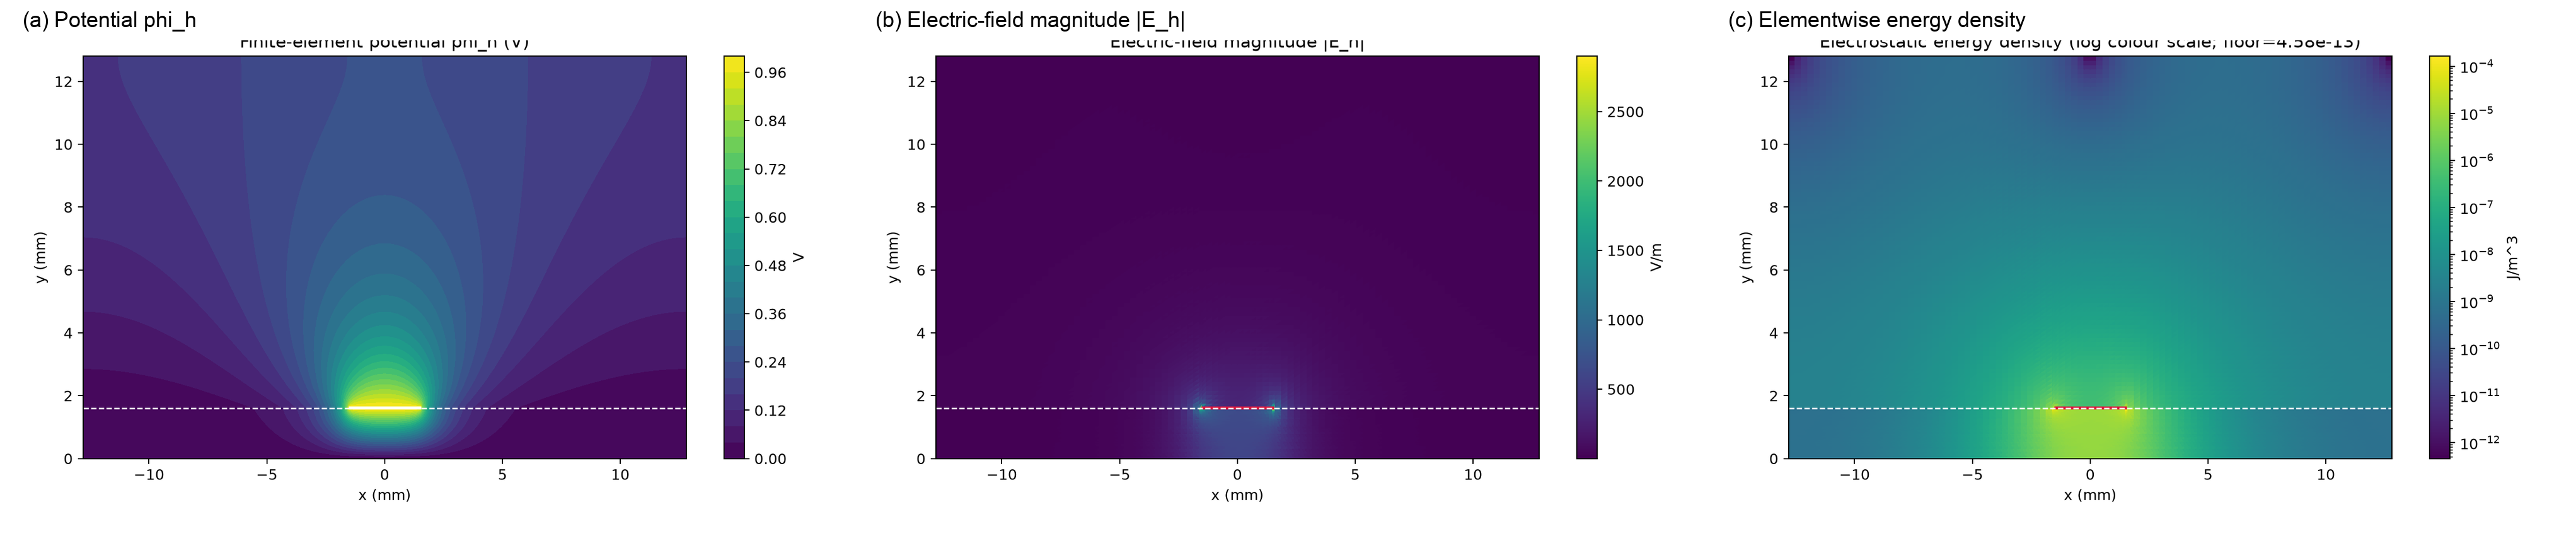
\includegraphics[width=\textwidth]{baseline_field_diagnostics.png}
\caption{Baseline field diagnostics on the production $8H$ domain: (a) finite-element
potential $\phi_h$, (b) electric-field magnitude $|\mathbf{E}_h|$ with
$\mathbf{E}_h=-\nabla\phi_h$, and (c) elementwise electrostatic energy density
$\tfrac12\varepsilon|\mathbf{E}_h|^2$ (J/m$^3$), shown with a logarithmic colour scale for
visibility. The potential respects the imposed Dirichlet values, while the field and the
energy density concentrate near the trace corners; away from the trace the box is quiescent.
These plots are diagnostic visualisations, not error norms.}
\label{fig:field}
\end{figure}

\subsection{The corner sets the rate}
The point is the corner marked in Figure~\ref{fig:geometry}, where the conductor edge
terminates on the dielectric interface. There the local solution behaves like
$r^{\alpha}$ with $\alpha<1$, so the gradient is unbounded and the usual
$h^{p}$-type estimate does not apply. Fitting $\phi_h$ along rays from each of the four
trace corners on the two finest meshes gives a median exponent
$\alpha=\CornerAlpha$ (range $\CornerAlphaLo$--$\CornerAlphaHi$ across corners and levels).
The exponent has a field consequence that does not depend on the fit: if the potential
behaves like $r^{\alpha}$ then $|\nabla\phi|$ behaves like $r^{\alpha-1}$, so the peak value
keeps moving under refinement instead of settling. That is visible in
Figure~\ref{fig:field}(b), where the saturated core is one or two elements wide at every mesh
size used here, and it is why no local field strength is reported as a design quantity: the
number belongs to the discretisation, not to the device.

For a quadratic functional of the solution the expected rate is $2\alpha$, so
$\CornerTwoAlpha$ is the prediction to set against the measured $\OrderPOne$. The match is of
the right order rather than exact, and it cannot be better: the constant multiplying the
singular term, the mixture of four corners with different exponents and the dielectric
interface all enter the prefactor, and the fit window is not asymptotic. What the comparison
does establish is the mechanism, since the measured rate is neither one nor two but twice a
corner exponent strictly between $0$ and $1$. The same value holds for both element families,
because both resolve the same singularity.

\section{Corner Grading}
\subsection{What is refined, and what is not}
If the error is generated at the corners, the mesh should be fine there and coarse
elsewhere. Figure~\ref{fig:mesh} makes that visible on a pair of meshes small enough to
see: the uniform M2 mesh and the graded G2 mesh in the same window, then the same pair
enlarged at the right-hand trace end. G2 costs $1{,}422$ unknowns against $404$ for M2,
and every extra element sits within a few hundred micrometres of the four corners. The
middle of the trace and the far field are the same elements in both pictures. That is the
whole claim of grading, separated from any question of cost: it moves resolution, it does
not add physics.

\begin{figure}[H]
\centering
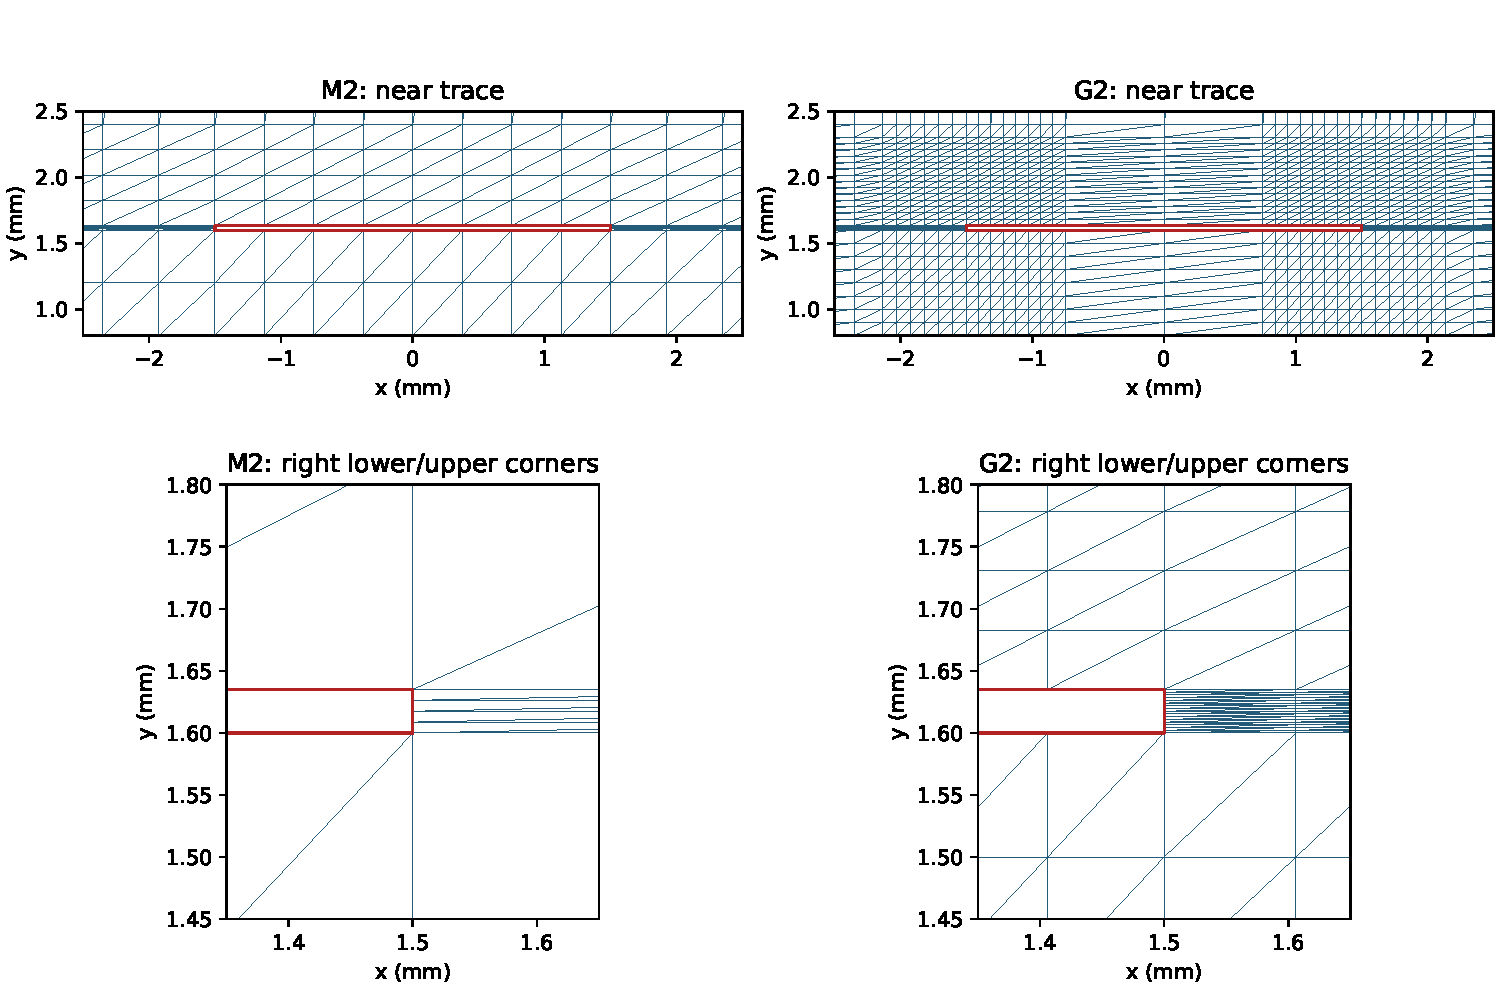
\includegraphics[width=\textwidth]{uniform_graded_corner_mesh.pdf}
\caption{What grading changes and what it leaves alone. Top row: uniform M2 and graded G2
in the same window near the right-hand trace end. Bottom row: the same pair enlarged at
the corner. The two meshes differ only within a few hundred micrometres of the corner:
G2 has $1{,}422$ unknowns against $404$ for M2, and every extra element is spent there.
These are geometry views and not a matched-DOF efficiency claim.}
\label{fig:mesh}
\end{figure}

The same rule drives the production run. On the fixed M5 background, round $k$ marks the
elements within $r_0 0.35^{\,k-1}$ of a corner, with $r_0=1.6\times10^{-4}\,\mathrm{m}$,
and the marked elements are refined by newest-vertex bisection with a symmetry completion
that keeps the mesh conforming about $x=0$. Nothing else changes: the operator, the
boundary conditions, the extraction and the material tags are those of
Algorithm~\ref{alg:fem}. Seven rounds of this produce the mesh behind the numbers in
Section~\ref{sec:grading-worth}, and at the seventh round the corner elements are about
$0.3\,\mu$m across, which is under one printed pixel at the width of a page. That is why
Figure~\ref{fig:mesh} shows the two-round mesh: the last rounds are visible as a number,
not as a picture.



\subsection{The plateau moves with the background}
The graded error does not fall to zero on a fixed background. It stalls at a plateau set by
the resolution far from the corner, and repeating the same seven rounds on four backgrounds
separates the two contributions: the plateau falls by a factor of about four per background
level (Table~\ref{tab:graded}).

\begin{table}[H]
\centering
\small
\caption{Final error after the same grading campaign on four backgrounds. The plateau ratio
is the previous row divided by the current one; a value near four is the signature of an
$h^2$ error in the far field.}
\label{tab:graded}
\begin{tabular}{@{}lrrrr@{}}
\toprule
Background & final DOFs & error (\%) & plateau ratio & DOFs ratio\\
\midrule
M2 & 2{,}560 & \GradedBTwo & -- & --\\
M3 & 9{,}772 & \GradedBThree & \PlateauOne & 3.82\\
M4 & 36{,}396 & \GradedBFour & \PlateauTwo & 3.72\\
M5 & \GradedDof & \GradedBFive & \PlateauThree & 3.83\\
\bottomrule
\end{tabular}
\end{table}

The plateau ratios ($\PlateauOne$, $\PlateauTwo$, $\PlateauThree$) are constant, so the
residual error is a second-order error of the background mesh and not a numerical floor.
Because the unknowns grow by the same factor as the plateau falls, one further order of
magnitude costs a full background refinement: grading buys a constant factor, not a better
rate.

\subsection{What the grading is worth}
\label{sec:grading-worth}
On the M5 background the campaign ends at $\GradedDof$ unknowns with
$\GradedErr\%$, against $\DofSeven$ unknowns and $\ErrSeven\%$ for uniform M7. That is
$\GradedRatio\times$ closer at $\GradedDofFrac\%$ of the unknowns, and it is the reason the
graded value is reported as an alternative discretisation of the same model. It is not
substituted for the M7 value: the submitted capacitance is the uniform one, because that is
the sequence against which the reference in Section~4 was built, and mixing the two would
destroy the error attribution the rest of the report depends on. The campaign behind these
numbers, including what happens on the other three backgrounds, is Figure~\ref{fig:graded}.

\begin{figure}[htbp]
\centering
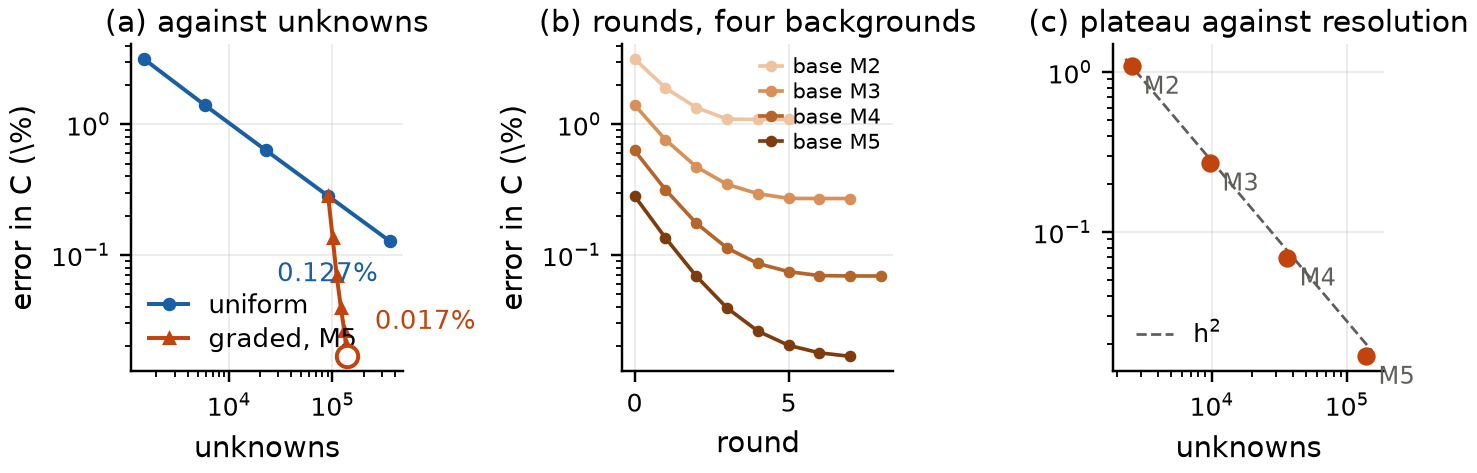
\includegraphics[width=\textwidth]{fig_cost_campaign.png}
\caption{The campaign on three axes. (a)~Error in $C$ against unknowns for both families: the
graded sequence ends at $\GradedDof$ unknowns and $\GradedErr\%$, the uniform M7 point at
$\DofSeven$ unknowns and $\ErrSeven\%$. (b)~The same seven rounds repeated on four backgrounds,
which stall at a plateau instead of reaching zero. (c)~That plateau against the resolution of
its own background, with the $h^2$ reference line: the plateau follows the background, not the
number of rounds.}
\label{fig:graded}
\end{figure}

\section{Residual-Based Adaptive Refinement}
\label{sec:adaptive}
\subsection{A second error measure, declared first}
Grading is a rule we imposed. The alternative is to let the computed solution choose the
elements, so this section runs a residual-based adaptive campaign on the same problem and
compares it with uniform and graded refinement. One thing must be said before any number is
quoted: this section measures a different quantity from Sections~4 and~7. The capacitance
experiment asks how far the computed $C$ is from the Richardson limit, in per cent; the
experiment here asks how far the computed potential is from a frozen reference solution, in
the energy norm. A small energy error does not imply a small capacitance error, and the
meshes, the starting points and the stopping rules all differ. Every number below is an
energy-norm number, and nothing here changes the submitted capacitance.

\begin{table}[H]
\centering
\footnotesize
\caption{The two error measures of this report, kept apart: they answer different
questions and are not interchangeable.}
\label{tab:two-metrics}
\begin{tabular}{@{}p{1.7cm}p{5.9cm}p{6.6cm}@{}}
\toprule
 & Energy norm (Section~\ref{sec:adaptive}) & Capacitance (Sections~4 and~7)\\
\midrule
Error & $E_{{\rm rel},M6}=\|e_{M6}\|_E/\|\phi_{M6}\|_E$ & $|C_h-C_{\rm ref}|/C_{\rm ref}$\\[1.5pt]
Reference & frozen M6 and M7 solutions & Richardson limit of the $12H$ family\\[1.5pt]
Setting & M1-S start, $\theta=0.5$, eight cycles & M5 background, seven rounds; uniform M2--M7\\
\bottomrule
\end{tabular}
\end{table}

\subsection{Where the indicator puts the elements}

\begin{figure}[H]
\centering
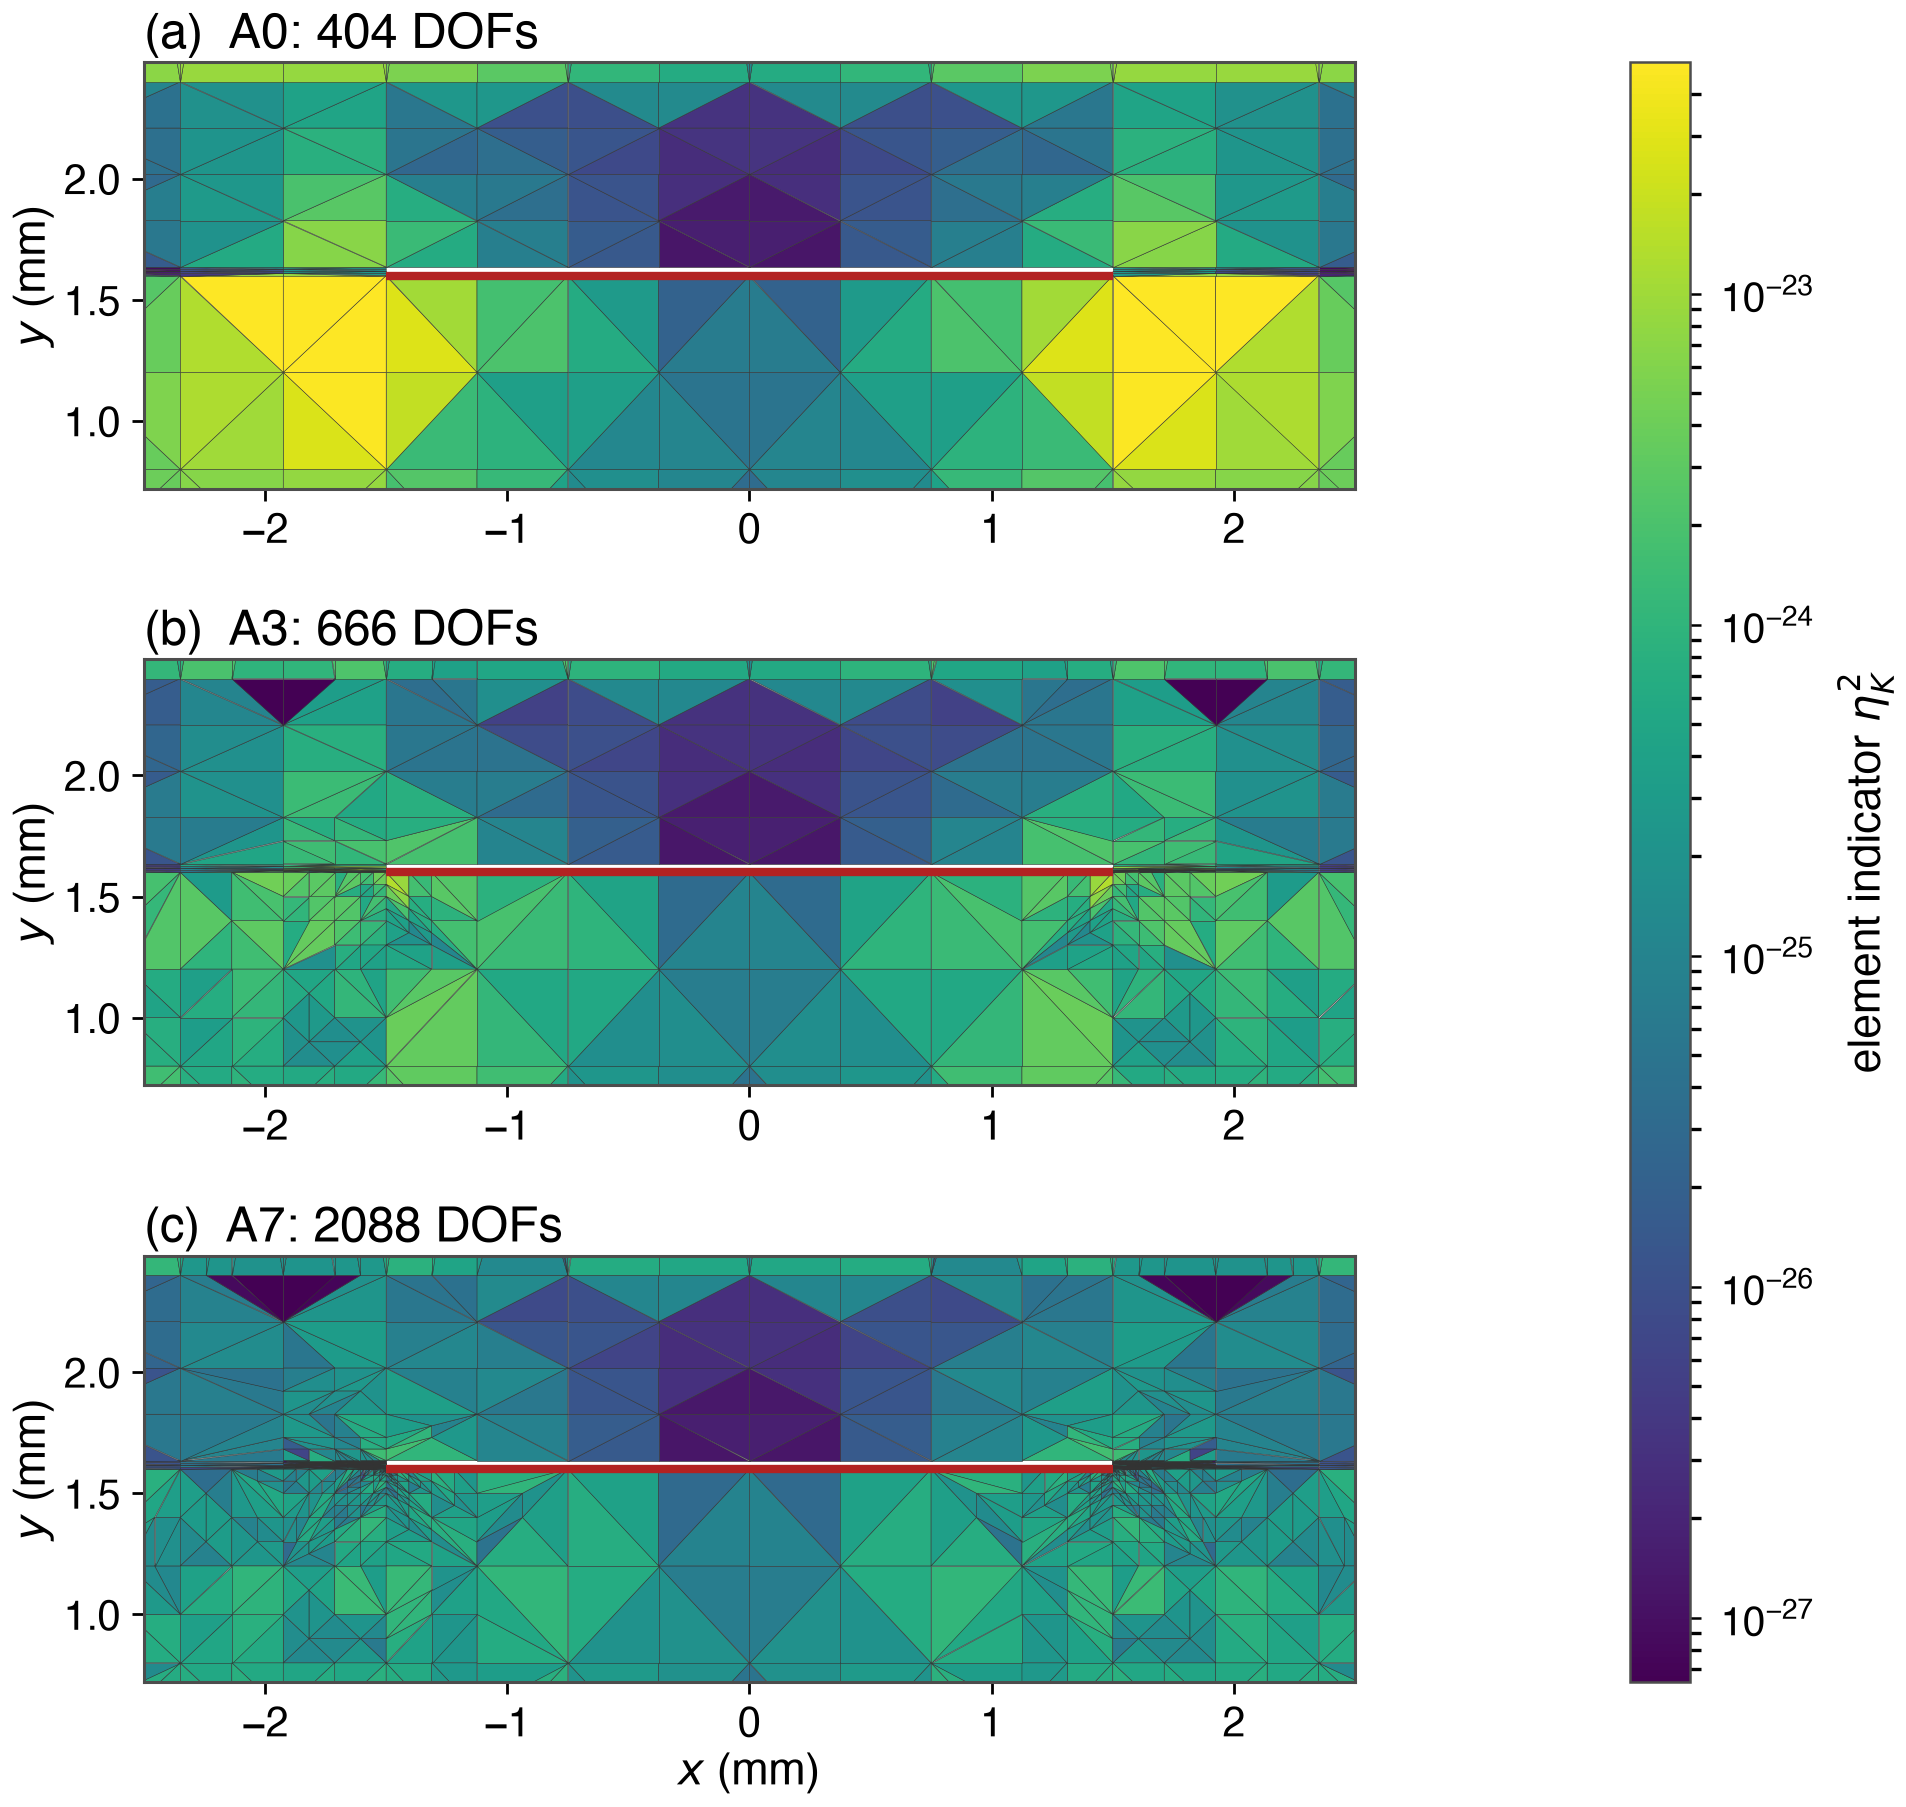
\includegraphics[width=0.74\textwidth]{fig_adaptive_meshes.png}
\caption{Where the indicator puts the resolution: the A0, A3 and A7 meshes in the same
physical window near the right-hand trace end, with the conductor edge in red. Element
colours show $\eta_K^2$ on one shared logarithmic scale, so the three panels are directly
comparable. Refinement collects at the trace ends, but not only there: marked elements also
appear in the substrate and in the air above the corner. This is observed localisation, not
a claim that the indicator identifies every singular contribution.}
\label{fig:adaptive-mesh}
\end{figure}

For $f=0$, constant elementwise $\epsilon$ and affine $\phi_h|_K$ the interior volume
residual vanishes, so the indicator is built entirely from the jumps of the flux across
interior edges,
\[
\eta_K^2=\frac12\sum_{e\subset\partial K\cap\mathcal E_{\rm int}}h_e\|J_e\|_{L^2(e)}^2,
\qquad
J_e=(\epsilon\nabla\phi_h|_{K^+}-\epsilon\nabla\phi_h|_{K^-})\cdot n_e ,
\]
with one normal $n_e$ used on both sides and interface edges included. This is a residual
indicator, not a guaranteed error bound. At every cycle the elements are sorted by
$\eta_K^2$ and the smallest prefix carrying at least $\theta=0.5$ of $\sum_K\eta_K^2$ is
refined; reflected elements are added to keep the mesh symmetric about $x=0$, and every
split edge is closed so that the triangulation stays conforming. Eight cycles are run from
a symmetry-completed M1 start with $404$ unknowns.


Within $0.25H$ of a trace corner the element fraction rises from $5.11\%$ at A0 to $62.0\%$
at A7, and those elements carry $79.6\%$ of the final squared indicator; the far boundary
carries $0.00265\%$ of it, so no resolution is being wasted on the outside box. Two features
of Figure~\ref{fig:adaptive-mesh} are worth naming. The refinement is not confined to the
four corners we would have picked by hand: marked centroids reach $|x|=5.0$\,mm and
$y=4.57$\,mm, outside the corner disks, because the substrate and the air above the trace
end carry a real flux imbalance too. And the concentration is strongest early. At A0,
$88.6\%$ of the indicator already sits in elements whose nearest corner is a lower
junction; by A7 that fraction has fallen to $50.2\%$, so lower-junction dominance is an
early-cycle effect rather than a permanent property of the indicator.

\subsection{What it buys, and what it costs}
\begin{figure}[H]
\centering
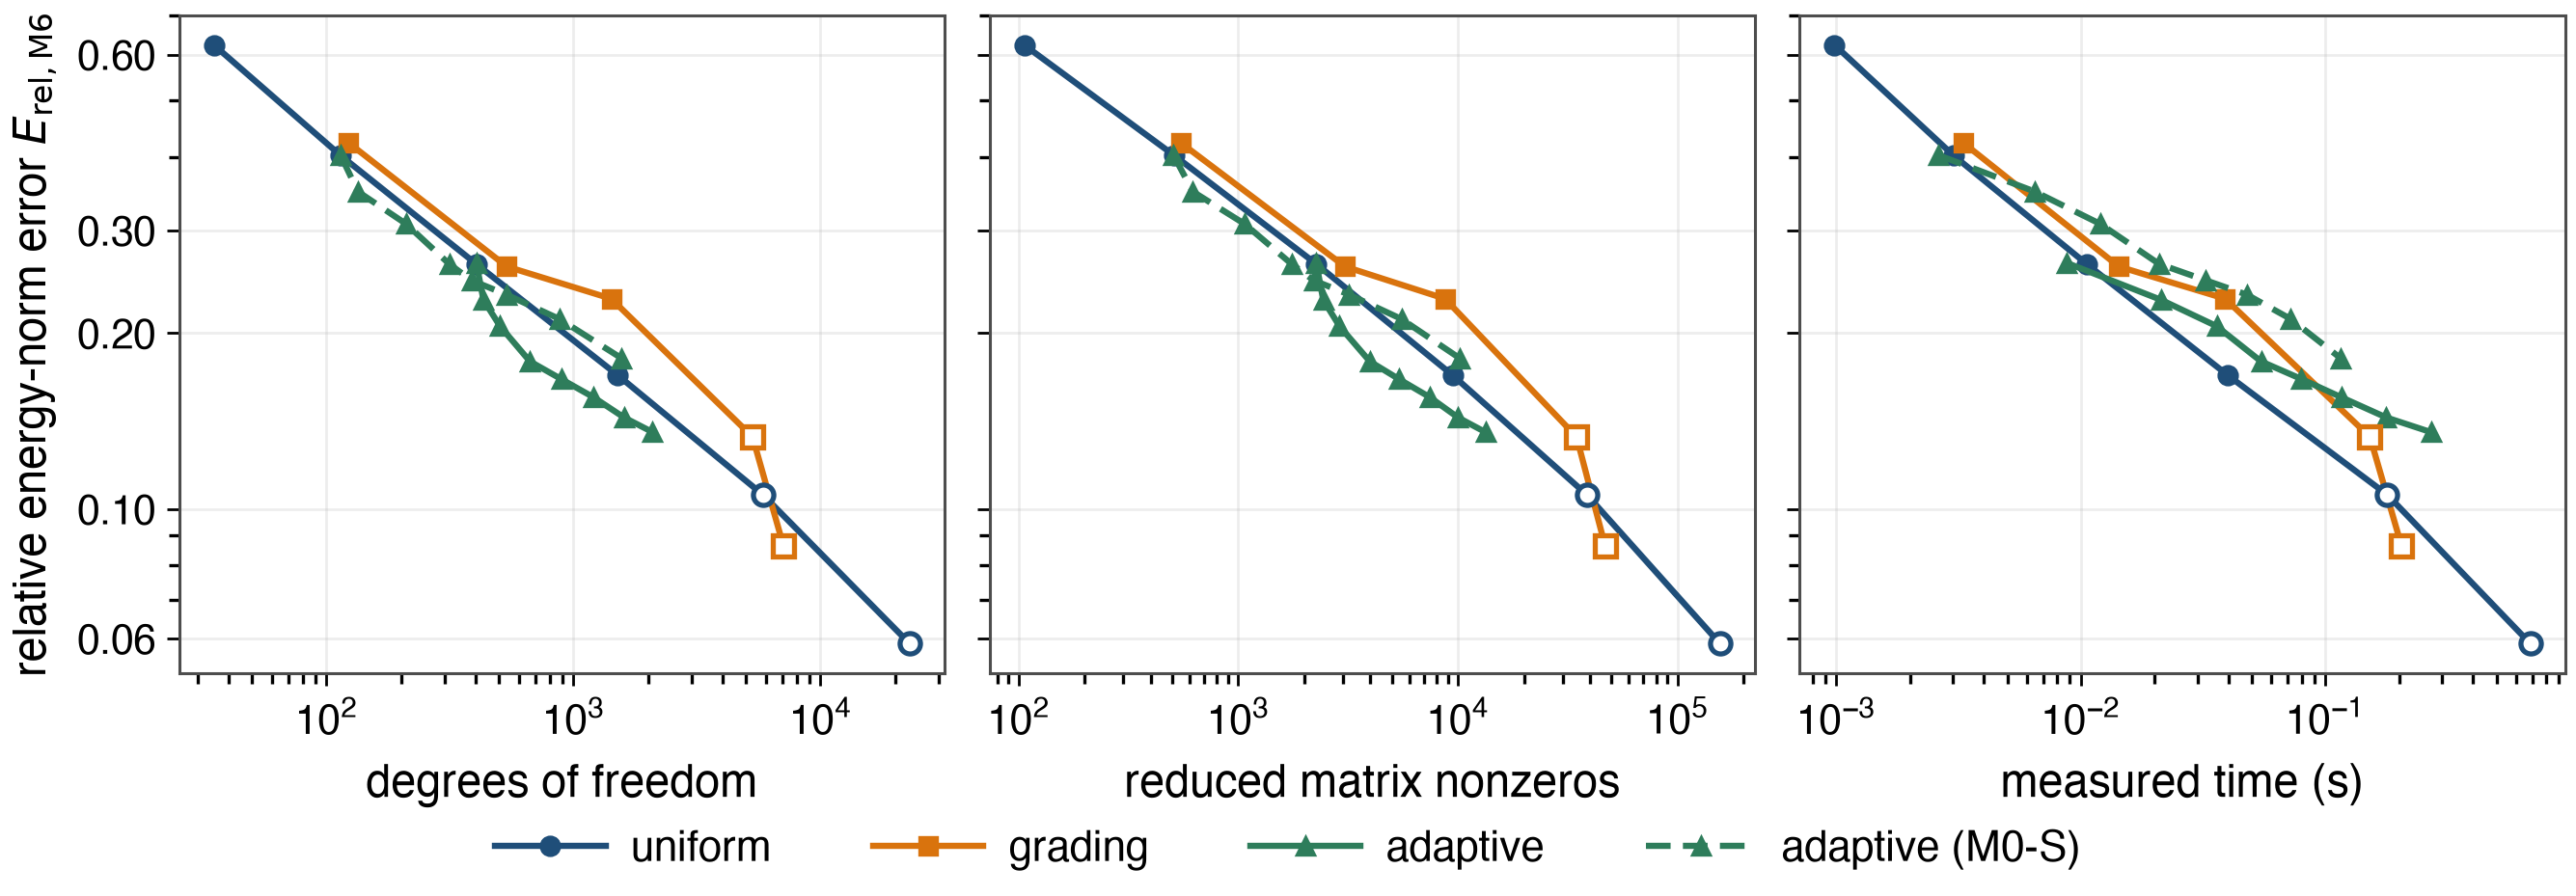
\includegraphics[width=\textwidth]{fig_adaptive_work.png}
\caption{All three refinement strategies in one error measure, $E_{\rm rel,M6}$, against
(a)~unknowns, (b)~reduced matrix nonzeros and (c)~measured median total algorithm time.
Adaptive work is cumulative from its initial mesh, so each point contains every preceding
solve, estimate, mark and refine cycle. Open markers fail the $3\%$ M6/M7
reference-sensitivity test and are shown for completeness, not for formal comparison.}
\label{fig:adaptive-work}
\end{figure}

Panel~(a) is the flattering one for adaptivity. At a common target of $E_{\rm rel}=0.30$ the
adaptive path needs about $224$ unknowns against $273$ for uniform refinement and $349$ for
grading, so the DOF ratio is $1.218$ and the nonzero ratio $1.235$ in its favour. Panel~(c)
is the other half of the same experiment: at that target the cumulative median time is
$13.1$\,ms for the adaptive path against $7.15$\,ms for uniform and $9.30$\,ms for grading.
Adaptivity wins on unknowns and loses on time, by a factor of about $1.8$ against uniform.

The direct comparison, which needs no interpolation, says the same. A5 reaches
$E_{\rm rel}=0.1553$ with $1{,}206$ unknowns while uniform M3 reaches $0.1694$ with
$1{,}512$: adaptive is $20\%$ smaller and takes $2.9$ times the cumulative time. Nor is the
advantage in unknowns uniform along the curve. At $E_{\rm rel}=0.40$ the DOF ratio is
$1.013$, which is no saving at all, and at the fine end A7 needs $2{,}088$ unknowns where
uniform M3 already had $1{,}512$ at a comparable error.

The mechanism is in how the work is counted, and it is not a bookkeeping convention. A
uniform mesh is one mesh: generate, assemble, solve once. An adaptive path is eight solves,
seven estimator evaluations, seven marking passes and seven refinements, and the cumulative
time at cycle $k$ contains all of them, because all of them are needed to obtain the mesh
that produced the error at cycle $k$. The saving in memory is real, since the final adaptive
mesh is smaller than the uniform mesh of the same error. The cost in time is equally real,
because the coarse solves cannot be skipped to reach the fine one. At millisecond scale none
of this separates cleanly from machine noise, so the claim is kept qualitative: residual
adaptivity reduces unknowns on this problem, and it does not reduce wall time.

For the report the practical consequence is that grading remains the working method. It is
a rule that fits in one line, it needs no reference solution to run, and it costs one mesh
generation and one solve. The adaptive campaign is kept for a different reason: it locates
the error without using our own guess about where the error is, and it agrees with that
guess.

\section{Algebraic Error}
\subsection{A ladder of tolerances}
Every number so far is a discretisation error, which assumes the linear systems are solved
exactly enough not to matter. That assumption is tested rather than asserted. On M5 the
sparse direct solve is replaced by conjugate gradients with relative tolerances from
$10^{-2}$ to $10^{-12}$, and the resulting change in $C$ is compared with the
discretisation error on the same mesh, $\TolDisc$.

\begin{figure}[htbp]
\centering
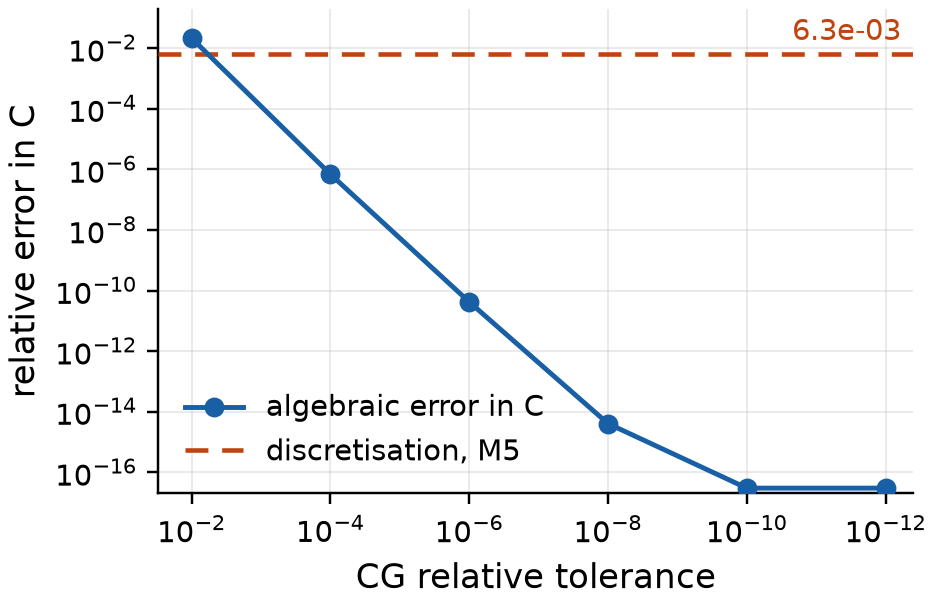
\includegraphics[width=0.63\textwidth]{fig08_tolerance.png}
\caption{Algebraic error in $C$ against the CG stopping tolerance on M5. The error follows
the tolerance until about $10^{-8}$ and then stops, at which point the discretisation error
of the mesh is the only thing left.}
\label{fig:tolerance}
\end{figure}

\begin{table}[H]
\centering
\small
\caption{Stopping tolerance against the induced error in $C$ on M5. The last column
compares it with the discretisation error of the same mesh.}
\vspace{6pt}
\label{tab:tolerance}
\begin{tabular}{@{}lrrr@{}}
\toprule
CG rtol & error in $C$ & scaled residual & error / $\TolDisc$\\
\midrule
$10^{-2}$ & $\TolAlgebraicAtCoarse$ & $9.4\times10^{-3}$ & $3.4$\\
$10^{-4}$ & $6.9\times10^{-7}$ & $5.2\times10^{-5}$ & $1.1\times10^{-4}$\\
$10^{-6}$ & $4.2\times10^{-11}$ & $1.1\times10^{-6}$ & $6.7\times10^{-9}$\\
$10^{-8}$ & $4.1\times10^{-15}$ & $5.7\times10^{-9}$ & $6.4\times10^{-13}$\\
$10^{-10}$ & $0$ & $6.2\times10^{-11}$ & $0$\\
\bottomrule
\end{tabular}
\end{table}

Once the tolerance is below $10^{-8}$ the two errors are separated by about thirteen orders of
magnitude: the algebraic contribution sits at the roundoff floor, $\TolAlgebraicFloor$, while
the discretisation error is $\TolDisc$. Tolerance is not irrelevant, since at $10^{-2}$ the
algebraic error is three times the discretisation error and would corrupt every number in
Section~5, but at the default setting it is a solved problem and the remaining error budget
belongs to the corner.

\section{Domain Truncation}
\label{sec:truncation}
The unbounded air region is approximated by a finite rectangle with a zero-flux outer
boundary. To isolate the effect we used the sequence
$(W/H,H_{\mathrm{air}}/H)=(3,3),(5,5),(8,8),(12,12)$ while preserving the near-trace mesh,
and repeated the largest domain with a finer near-field resolution to separate truncation
from mesh resolution.

\begin{table}[H]
\centering
\small
\caption{Domain-truncation sequence. The last row repeats $12H$ with a finer near field to
show that the $12H$ value is itself resolved to better than $0.04\%$.}
\label{tab:truncation}
\begin{tabular}{@{}rrrrr@{}}
\toprule
$W/H=H_{\mathrm{air}}/H$ & Elements & DOFs & $C_E$ (pF/m) & difference from $12H$\\
\midrule
3 & 11868 & 6121 & 118.839 & $\TruncThree\%$\\
5 & 16988 & 8711 & 121.004 & $\TruncFive\%$\\
8 & 26168 & 13346 & 121.653 & $\TruncEight\%$\\
12 & 41208 & 20926 & 121.875 & reference\\
12 (refined) & 60720 & 30741 & 121.831 & $\TruncFine\%$\\
\bottomrule
\end{tabular}
\end{table}

The $8H$ box costs $\TruncEight\%$, the same size as the discretisation error at M7
($\ErrSeven\%$).

\begin{figure}[htbp]
\centering
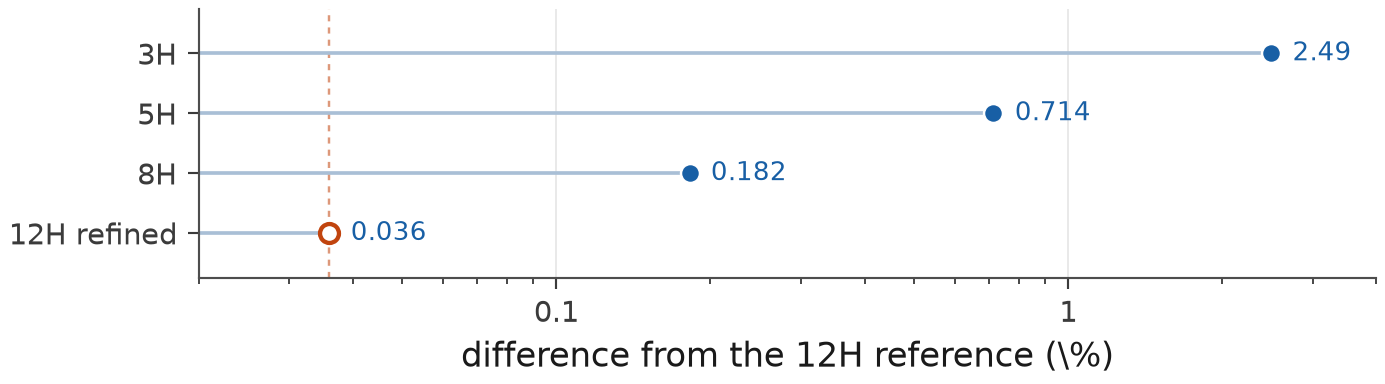
\includegraphics[width=\textwidth]{fig09_truncation.png}
\caption{Difference from the $12H$ reference for each domain. The open marker and the dashed
line mark the refined $12H$ repeat, whose $0.036\%$ is the mesh-noise floor. On a logarithmic
scale the decay is close to exponential in the box size before it flattens at that floor.}
\label{fig:truncation}
\end{figure}

Two caveats qualify that statement rather than sit in a footnote. The $8H$ and
$12H$ values in Table~\ref{tab:truncation} are production meshes at their own resolutions, so
their difference mixes truncation with mesh resolution; the refined $12H$ repeat puts the
latter at $\TruncFine\%$, which is why the $0.18\%$ is attributed mainly to truncation. And the
M7 value of Section~11 is not on this sequence at all, so $0.18\%$ measures the sensitivity of
the answer to the domain choice; it is not a measured truncation error for the submitted
value. It is quoted beside the discretisation error to show that the two are comparable, not
to be added to it.

\section{Final Values}
\label{sec:final}
\subsection{Capacitance and its distance from the limit}
The submitted dielectric capacitance is the M7 value,
\begin{equation}
C_{M7}=\CFinal\ \mathrm{pF/m},
\label{eq:cfinal}
\end{equation}
and its distance from the extrapolated limit $C_{\rm ref}=\CRef\,\mathrm{pF/m}$
of~\eqref{eq:cref} is
\begin{equation}
C_{M7}-C_{\rm ref}=\CFinalAbs\ \mathrm{pF/m},
\label{eq:cminref}
\end{equation}
which is $\ErrSeven\%$ of $C_{\rm ref}$.
Both numbers are written out rather than folded into a $\pm$ interval, because $0.153$ is
not an uncertainty: the M7 solve is deterministic and repeatable, and the gap is what the
mesh resolution still costs against the limit. The finite box adds a separate sensitivity of
$\TruncEight\%$, discussed in Section~\ref{sec:truncation}, which is of the same size; the
two are reported side by side and are never added into one error bar. The all-air run reuses
the exact frozen M7 mesh --- same nodes, same boundary sets, same sparsity pattern, only the
material tags changed --- giving $\Cair=\CAir\,\mathrm{pF/m}$, which is $\CAirErr\%$ above
its own extrapolated limit of $\CAirRef\,\mathrm{pF/m}$.

\begin{figure}[htbp]
\centering
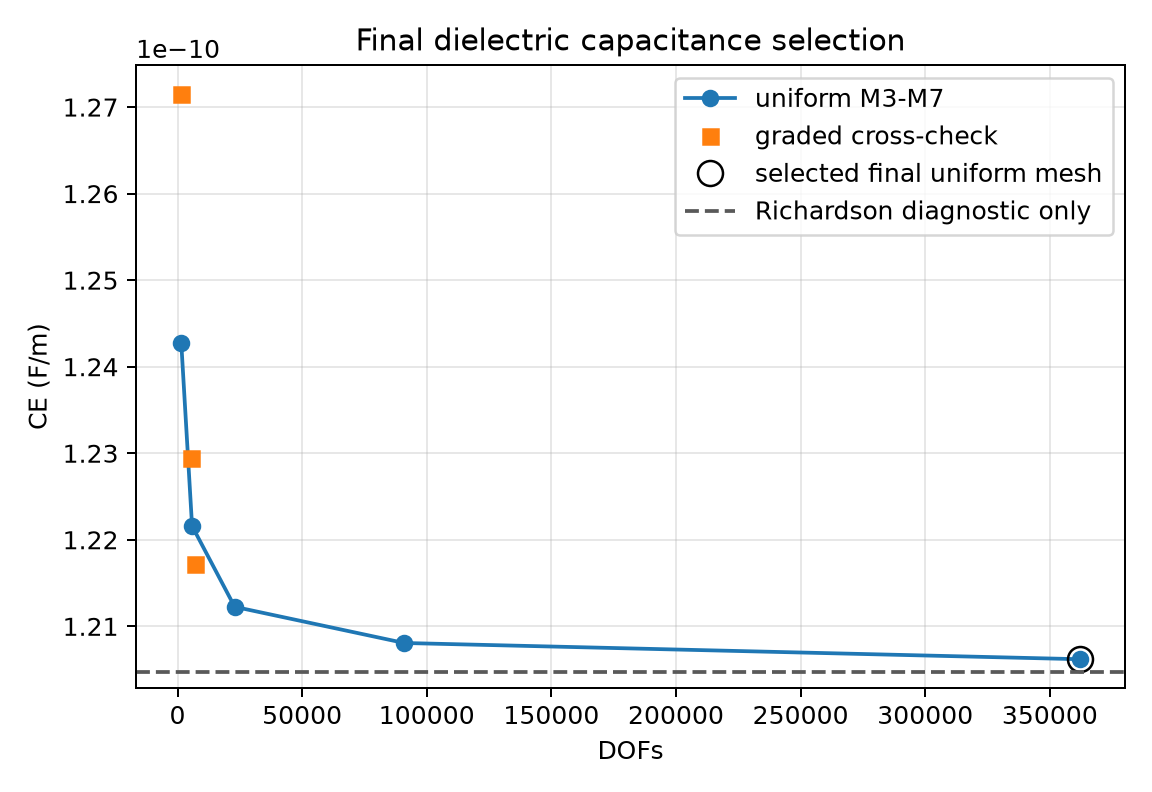
\includegraphics[width=0.68\textwidth]{final_capacitance_convergence.png}
\caption{Final dielectric capacitance selection. M7 is the selected computed FEM mesh; the
graded run is an independent cross-check on the same quantity, and the Richardson line is a
diagnostic only.}
\label{fig:finalcap}
\end{figure}

Reusing the mesh is not a convenience. If the all-air case were remeshed, the ratio
$C/\Cair$ would contain a mesh difference as well as a material difference, and the
effective permittivity would inherit an error that no convergence study of $C$ alone could
detect. The mesh fingerprint is checked before the air run, so the material change is the
only difference between the two systems.

\subsection{Effective permittivity}
The ratio
\begin{equation}
\epseff=\frac{C}{\Cair}=\EpsEff
\label{eq:epseff}
\end{equation}
is to be compared with the exact ratio of the two limits, $\EpsRef$. The discrepancy is
$\EpsErr\%$, about half the $\ErrSeven\%$ error of $C$ itself, because the two errors are
strongly correlated: both meshes share the same corner under-resolution, and dividing
removes the common part. The improvement is real, but it is not independent information. The
same bias is cancelling, not being measured twice.

\subsection{Characteristic impedance}
With $c_0$ the vacuum speed of light, the quasi-TEM relations give
\begin{equation}
L=\frac{1}{c_0^2\Cair},\qquad
\Zzero=\sqrt{\frac{L}{C}}=\frac{1}{c_0\sqrt{C\,\Cair}}
=\frac{1}{c_0\Cair\sqrt{\epseff}} .
\label{eq:z0}
\end{equation}
The three expressions agree to floating-point precision, which is an internal identity and
not a validation. Numerically, $\Zzero=\ZFinal\,\Omega$ against $\ZRef\,\Omega$ from the
reference pair, a difference of $\ZErrAbs\,\Omega$ or $\ZErrPct\%$.

\begin{figure}[htbp]
\centering
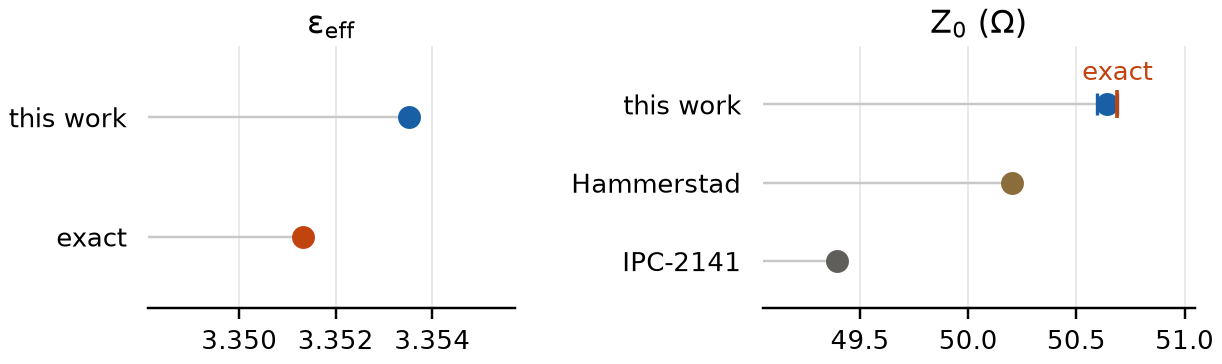
\includegraphics[width=0.84\textwidth]{fig11_engineering.png}
\caption{The two engineering quantities against their exact counterparts and the
independent formulas. Left: $\epseff$ against the ratio of the extrapolated limits. Right:
$\Zzero$ with the reference marked; the horizontal bar is the propagated uncertainty from
the capacitance pair, not a confidence interval.}
\label{fig:engineering}
\end{figure}

\begin{table}[H]
\centering
\small
\caption{Engineering benchmark comparison. The primary $d_{\rm HJ}$ column uses the
Hammerstad--Jensen value in the denominator, as specified; the last column is the
supplementary difference normalised by the FEM value and is not $d_{\rm HJ}$.}
\label{tab:bench}
\begin{tabular}{@{}lrrrr@{}}
\toprule
Method & $\varepsilon_{\rm eff}$ & $Z_0$ ($\Omega$) & $100d_{\rm HJ}$ & Diff. vs FEM\\
\midrule
FEM matched pair & 3.3535 & 50.642 & $0.879\%$ & $0.000\%$\\
Hammerstad--Jensen & 3.3008 & 50.201 & $0.000\%$ & $0.871\%$\\
IPC-2141 & -- & 49.393 & $1.608\%$ & $2.466\%$\\
\bottomrule
\end{tabular}

\end{table}

The Hammerstad--Jensen formula gives $\ZHJ\,\Omega$ and IPC-2141 gives $\ZIPC\,\Omega$; the
two approximations differ from each other by $\ZBenchGap\,\Omega$, which is seventeen times
our own $\ZErrAbs\,\Omega$. That comparison is the useful one: the disagreement between
standard formulas, not the agreement of any one of them with the FEM value, sets the scale
at which an impedance can be claimed. The FEM result is also $0.642\,\Omega$ above the
common $50\,\Omega$ design target, a difference of $1.28\%$ that is design context rather
than a numerical reference.

\section{Limitations}
The model is electrostatic and quasi-TEM. It omits dielectric and conductor loss, surface
roughness, dispersion, radiation, solder mask and manufacturing tolerance; the conductors
are perfect. Those omissions are larger than the $0.1\%$ numerical question the report
answers, and no numerical refinement removes them.

Three numerical limitations are specific to this work. The reference of~\eqref{eq:cref} is an
extrapolation from two families that have not reached their asymptotic regime: it is the best
available limit rather than an exact value, and the agreement of the two routes bounds the
extrapolation error without proving it small. The $0.18\%$ domain figure measures the
sensitivity of the answer to the domain choice, obtained on production meshes, and is not a
measured truncation error of the M7 solution. The grading analysis establishes a
constant-factor gain on one background family under one marking rule and nothing further; it
does not establish optimality, and other rules were not tested.

The adaptive campaign of Section~\ref{sec:adaptive} is a limitation as well as a check. Its
numbers are energy-norm numbers measured against frozen M6/M7 references, not capacitance
numbers against the extrapolated limit, and the two experiments were not run at matched
targets. It reduced the unknown count at the accuracy levels of interest but not the total
runtime, which is why the submitted values rest on a single uniform mesh rather than on an
adaptive sequence. That is a deliberate refusal, recorded rather than omitted.

\section{Conclusions}
\begin{sloppypar}
On the studied cross-section the submitted values are
$C=\CFinal\,\mathrm{pF/m}$, $\CFinalAbs\,\mathrm{pF/m}$ below the extrapolated limit, and
$\Cair=\CAir\,\mathrm{pF/m}$ on the same M7 mesh, hence $\epseff=\EpsEff$ and $\Zzero=\ZFinal\,\Omega$. These sit
$\ErrSeven\%$, $\EpsErr\%$ and $\ZErrPct\%$ away from limits obtained by two independent
routes that agree to $\RefAgree$.
\end{sloppypar}

Four findings underpin the numbers. $\CheckCount$ analytic configurations are reproduced to
roundoff, including a separate audit of the Dirichlet row on non-zero boundary data. The usual
convergence indicator understates the error by the factor $2^{p}-1=\RatioChange$, because the
measured order is $\OrderPOne$ rather than one. That order is set by the corner and not by the
basis, since $P_2$ gives $\OrderPTwo$. And grading the corner reaches $\GradedErr\%$ with
$\GradedDof$ unknowns, $\GradedRatio\times$ closer than M7 at $\GradedDofFrac\%$ of its size,
with a plateau that falls fourfold per background level.

The remaining error is therefore understood rather than merely small: it is the
discretisation of one point, it can be bought down by concentrating elements there, and the
two other contributions --- truncation at $\TruncEight\%$ and algebraic error thirteen
orders below it --- are quantified separately so that none of them is hidden inside a single
quoted figure.

\bibliographystyle{plain}
\bibliography{references}

\appendix
\section{AI Transparency Audit}
We used AI/Codex for code scaffolding, plotting, workflow generation, documentation,
consistency checks and report drafting and revision. Every numerical claim below was
re-checked against stored output, and the checks are designed so that a wrong claim fails
loudly rather than degrading gracefully. The first four cases record assumptions, possible
falsifiers, evidence locations and decisions.

The audit follows the five-gate process required for AI-assisted solver work: formula
transcription checked against the project documents; structure and indexing tested through
geometry, material-region, boundary-node and degree-of-freedom checks; the formulation
verified by deriving the weak form, the elimination and the capacitance identities
explicitly; independent reproduction addressed by the manufactured solution, the layered
problem, the two-route reference and the boundary-row audit; and fragile results
interrogated through the domain, reference-stability, grading and tolerance studies rather
than accepted at face value.

\begin{longtable}{@{}L{0.22\textwidth}L{0.32\textwidth}L{0.36\textwidth}@{}}
\caption{Project-specific AI audit summary.}\label{tab:aiaudit}\\
\toprule
Component & Main risk & Verification evidence\\
\midrule
\endfirsthead
\toprule
Component & Main risk & Verification evidence\\
\midrule
\endhead
$P_1$ assembly and elimination & Incorrect assembly, boundary treatment or coefficient handling & $\CheckCount$ analytic configurations; manufactured solution; layered problem; boundary-row audit\\
Microstrip geometry & Trace hole, interface or boundary nodes misidentified & Geometry tests; full and near-trace figures; potential bounds and symmetry\\
Capacitance extraction & Reaction sign or trace-node summation error & $C_E/C_Q$ agreement at $10^{-15}$; charge-balance defect\\
Reference value & Extrapolation of a sequence that is not asymptotic & Two families with different elements and codes, agreeing to $\RefAgree$\\
Order diagnosis & Attributing a reduced rate to the wrong cause & $P_1$ and $P_2$ slopes compared; corner exponent fitted independently\\
Corner grading & Confusing a constant-factor gain with a better rate & Four backgrounds; plateau ratios constant at about four\\
Domain study & Changing the far field also changes the near-trace mesh & Fixed near field; refined $12H$ repeat separates mesh from truncation\\
Final capacitance & Selecting a convenient mesh rather than an evidenced one & M3--M7 sequence; change-versus-error table; frozen mesh fingerprint\\
Matched all-air solve & Remeshing instead of changing only the material & Frozen mesh hash, same DOFs, same boundary sets, same sparsity pattern\\
Engineering benchmarks & Circular validation using FEM outputs inside the formulas & Benchmark functions accept only geometry and $\epsr$; formula spread quoted\\
\bottomrule
\end{longtable}

\paragraph{Case audit 1: energy--charge agreement.}
\noindent\textit{Claim examined:} near-equality of $C_E$ and $C_Q$ proves spatial
convergence.

\noindent\textit{Assumption:} both quantities use the same discrete potential, operator,
prescribed voltage and element integrals.

\noindent\textit{Risk and falsifier:} reactions and energy come from the same stiffness
matrix, so even a coarse mesh satisfies $2W_e=V_0Q_{\rm trace}$.

\noindent\textit{Independent evidence:} M3 has a $C_E/C_Q$ difference of
$1.0\times10^{-15}$ but $C_E=124.273\,\mathrm{pF/m}$, which is \ErrThree\% from the limit.

\noindent\textit{Decision:} reject the inference; use the energy--charge difference for
algebraic consistency and the mesh sequence for spatial sensitivity.

\paragraph{Case audit 2: the finite far boundary.}
\noindent\textit{Claim examined:} the tested $12H$ solution is the exact infinite-domain
answer.

\noindent\textit{Risk and falsifier:} a finite zero-flux boundary still perturbs the field,
so one large box cannot remove truncation.

\noindent\textit{Independent evidence:} the fixed-core $3H$--$12H$ sequence and the refined
$12H$ repeat separate the two effects; the repeat moves only $\TruncFine\%$ while the $8H$
difference is $\TruncEight\%$.

\noindent\textit{Decision:} call $12H$ a tested finite-domain reference and report
$\TruncEight\%$ as a sensitivity indicator, not a bound.

\paragraph{Case audit 3: errors across different meshes.}
\noindent\textit{Claim examined:} coefficient vectors from different meshes can be
subtracted elementwise.

\noindent\textit{Risk and falsifier:} vector entries live in different bases, and a fine
triangle crossing a coarse gradient jump invalidates constant-gradient integration.

\noindent\textit{Evidence:} in the earlier graded comparison, $21440$ of $180224$ reference
triangles crossed a coarse diagonal, about $4.55\%$ of the field-domain area.

\noindent\textit{Decision:} never subtract coefficients across meshes; transfer the coarse
gradient onto the reference elements and integrate there. The grading results of Section~7
use this route, and the earlier centroid-based curves are retained only as history.

\paragraph{Case audit 4: reading a plateau.}
\noindent\textit{Claim examined:} a graded error that stops falling has reached the
discretisation floor.

\noindent\textit{Risk and falsifier:} the plateau is set by the background mesh, not by
roundoff, so the same campaign on a finer background should keep falling.

\noindent\textit{Evidence:} four backgrounds give plateaus of
$\GradedBTwo\%$, $\GradedBThree\%$, $\GradedBFour\%$ and $\GradedBFive\%$, in constant ratio
$\PlateauOne$--$\PlateauThree$.

\noindent\textit{Decision:} report the grading gain as a constant factor tied to the
background, never as an improved rate; state the background whenever the graded error is
quoted.

\paragraph{Reproduction commands.}
The report and the slides share one number source. From the repository root:
\begin{verbatim}
python3 -m pip install -r requirements.txt
pytest -q
python3 presentation/make_figures.py   # figures + presentation/numbers.tex
python3 report/build_numbers.py        # report/numbers.tex
python3 report/make_field_figures.py   # field map and layered interface
python3 report/make_report_figures.py  # truncation and final-capacitance charts
python3 report/make_campaign_figures.py  # grading campaign, cost
python3 report/make_adaptive_figures.py  # adaptive meshes, three-way plot
cd report && latexmk -pdf main.tex     # or tectonic -X compile main.tex
python3 code_hardened/boundary_row_audit.py
\end{verbatim}
Most figures are produced by \path{presentation/make_figures.py} and copied unchanged into
\path{report/figures_v2/}, so a figure in the paper and the corresponding slide are the same
file. The field map, the layered-interface panels, the grading campaign, the adaptive mesh
snapshots and the three-way comparison are redrawn for the page by the four
\path{report/make_*.py} scripts listed above, from the same stored solves and numbers: the
adaptive panels read \path{results/adaptive_extension/meshes/A0,A3,A7.npz} and the cost
panels read \path{results/adaptive_extension/three_way_comparison.csv}. Timings vary between
runs; the numbers quoted here are those of the stored output.

\clearpage
\section{Individual Contribution Statements}

\begin{description}[style=nextline,leftmargin=0pt,labelwidth=0pt]
\item[Member 1:] \textbf{Chuqiao Tang (2360692)}. \todo{TO BE COMPLETED BY TEAM.}
\item[Member 2:] \textbf{Jinyu Ma (2363433)}. \todo{TO BE COMPLETED BY TEAM.}
\item[Member 3:] \textbf{Muqing Xu (2362900)}. \todo{TO BE COMPLETED BY TEAM.}

\item[Member 4:] \textbf{Shuoran Fu (2362626)}.

I worked on developing and organising the Python FEM code, including mesh generation,
boundary conditions, sparse matrix assembly and solution of the electrostatic problem. My
work covered files such as \path{code/geometry.py}, \path{code/fem_solver.py} and
\path{code/run_all.py}. I also worked on the numerical experiments: the verification suite,
the domain study, the uniform sequence and the reference value, and the corner-grading
campaign analysed in Section~7.

For the report, I designed the structure and wrote the technical sections in
\path{report/main.tex}, including the argument that separates the distance from the limit
from the change between meshes, and the diagnostics that attribute the reduced order to the
corner. I organised the figures and tables so that every number is produced by a script
from the stored tables.

AI tools assisted with coding, debugging and writing. I reviewed the generated content and
checked the numerical claims against the stored output. My main contribution was connecting
the implementation, the numerical experiments and the report into one consistent argument.

\noindent\textit{Repository evidence:} commits \texttt{2b9dfed}, \texttt{b5eee20} and
\texttt{7119103} record the code, report and frozen-mesh uploads under Shuoran Fu's account;
\texttt{c10eabf} and \texttt{ccd2f37} add the hardened verification suite and the
boundary-row audit. These are delivery records, not a complete record of individual work.

\item[Member 5:] \textbf{Taiqi Zhang (2363684)}. \todo{TO BE COMPLETED BY TEAM.}
\item[Member 6:] \textbf{Yujia Ding (2362094)}. \todo{TO BE COMPLETED BY TEAM.}
\end{description}

\end{document}
